\documentclass[9pt,twocolumn]{article}

\usepackage{graphicx}        % standard LaTeX graphics tool
\usepackage{subfig}

\begin{document}

\section{Evaluation}

\subsection{Experiment Setup}

Our experiments were conducted on a small LAN consisting of two laptops and two
workstations in the networks lab, all of which were connected by a small 10 Mbit
Ethernet hub. The lab workstations each ran an iperf client and an iperf server
in UDP mode, while our laptops each ran our chat client along with Wireshark.
One of our laptops also ran our chat server. Figure~\ref{fig:test_network} shows a
diagram of our test network.

\begin{figure*}[!t]
   \centering
      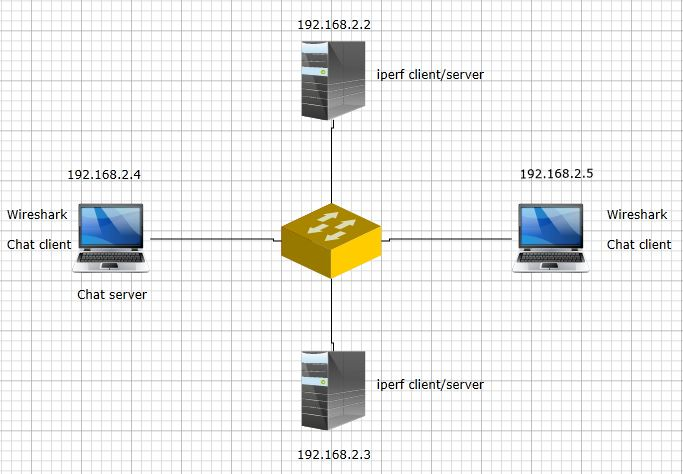
\includegraphics[width=0.8\textwidth]{pics/network_diagram}
   \caption{Test network diagram.}
\label{fig:test_network}
\end{figure*}

\subsection{Experiment Procedure}

Each of our test runs was conducted as follows. First, we started the iperf
clients and servers on the lab workstations and configured the clients to
generate the desired level of background traffic. Since both workstations were
running iperf clients, this resulted in cross-traffic flowing between the two
workstations. After initializing iperf, we started Wireshark captures on both of
our laptops. We then initiated a call between our chat clients, let the call
continue for 30 seconds, then aborted the call and saved both Wireshark
captures. We tested each protocol with the iperf clients sending 0, 9, and 10
Mbit/s of traffic, and each run was repeated a total of five times.

\subsection{Analysis Procedure}

In order to calculate packet losses, we used the Wireshark traces captured
during our experiments to determine how many packets were sent from one client
and received by the other. Specifically, we did this by applying this display
filter to both Wireshark traces from a particular session:\\

\texttt{(dccp|tcp|udp) and ip.src == 192.168.2.5 and data.len == 1407}\\

For the first term, we used the name of the protocol being used by our chat
program when the traces were captured. This expression filtered out all
packets except data packets that were sent from 192.168.2.5, one of our laptops.
For the trace recorded on 192.168.2.5, the number of displayed packets told us
how many packets were sent from 192.168.2.5.
Similarly, for the trace recorded on 192.168.2.4 (that is, the other chat
client), only data packets received from 192.168.2.5 were displayed. We
calculated the number of lost packets as the difference between these two
numbers.\\

We did not have a good way to directly measure network latency during our
experiments. Therefore, in order to analyze jitter, we measured delays between
incoming data packets. For each of our runs, we calculated the average delay
between consecutive pairs of incoming packets, and then calculated jitter as the
difference between an individual delay and the average delay. Finally, we
graphed the resulting jitter measurements as CDFs, with jitter on the X-axis and
the associated percentiles on the Y-axis.

\subsection{Discussion}

\subsubsection{Losses and Sending Rates}

As previously stated, we computed packet losses for each run. Our results are
shown in Figures ~\ref{fig:avg_losses}, ~\ref{fig:dccp_losses},
~\ref{fig:tcp_losses}, and ~\ref{fig:udp_losses}.\\

Unfortunately, our chat client proved unstable and crashed multiple times during
our UDP test runs. In an attempt to work around the issue, we tried starting our
Wireshark captures after initializing the voice call and the iperf clients. We
did our best to synchronize the start of our captures, but a handful of our UDP
captures were nevertheless out of sync and yielded invalid loss data. This is
why we have no packet loss data for UDP session 3 at 9 Mbit/s background
traffic. We acknowledge this was hardly an ideal solution, but we were unable to
troubleshoot the chat client effectively since William was largely unavailable
during our project's final stages.\\

It is interesting to note that, on average, DCCP dropped approximately 5\% more
packets at 9 Mbit/s of background traffic compared to 10 Mbit/s, whereas TCP and
UDP lost more packets at 10 Mbit/s than at 9 Mbit/s. We believe this may be a
result of DCCP's congestion control mechanism preemptively dropping packets in
order to avoid further congestion.  In contrast, TCP's congestion control is
primarily reactive (that is, it does not reduce its sending rate until the
network is oversaturated). UDP does not implement congestion control, so it
maintains its sending rate regardless of congestion, leading to proportionally
more losses at higher congestion levels.\\

\begin{figure}[h]
   \centering
      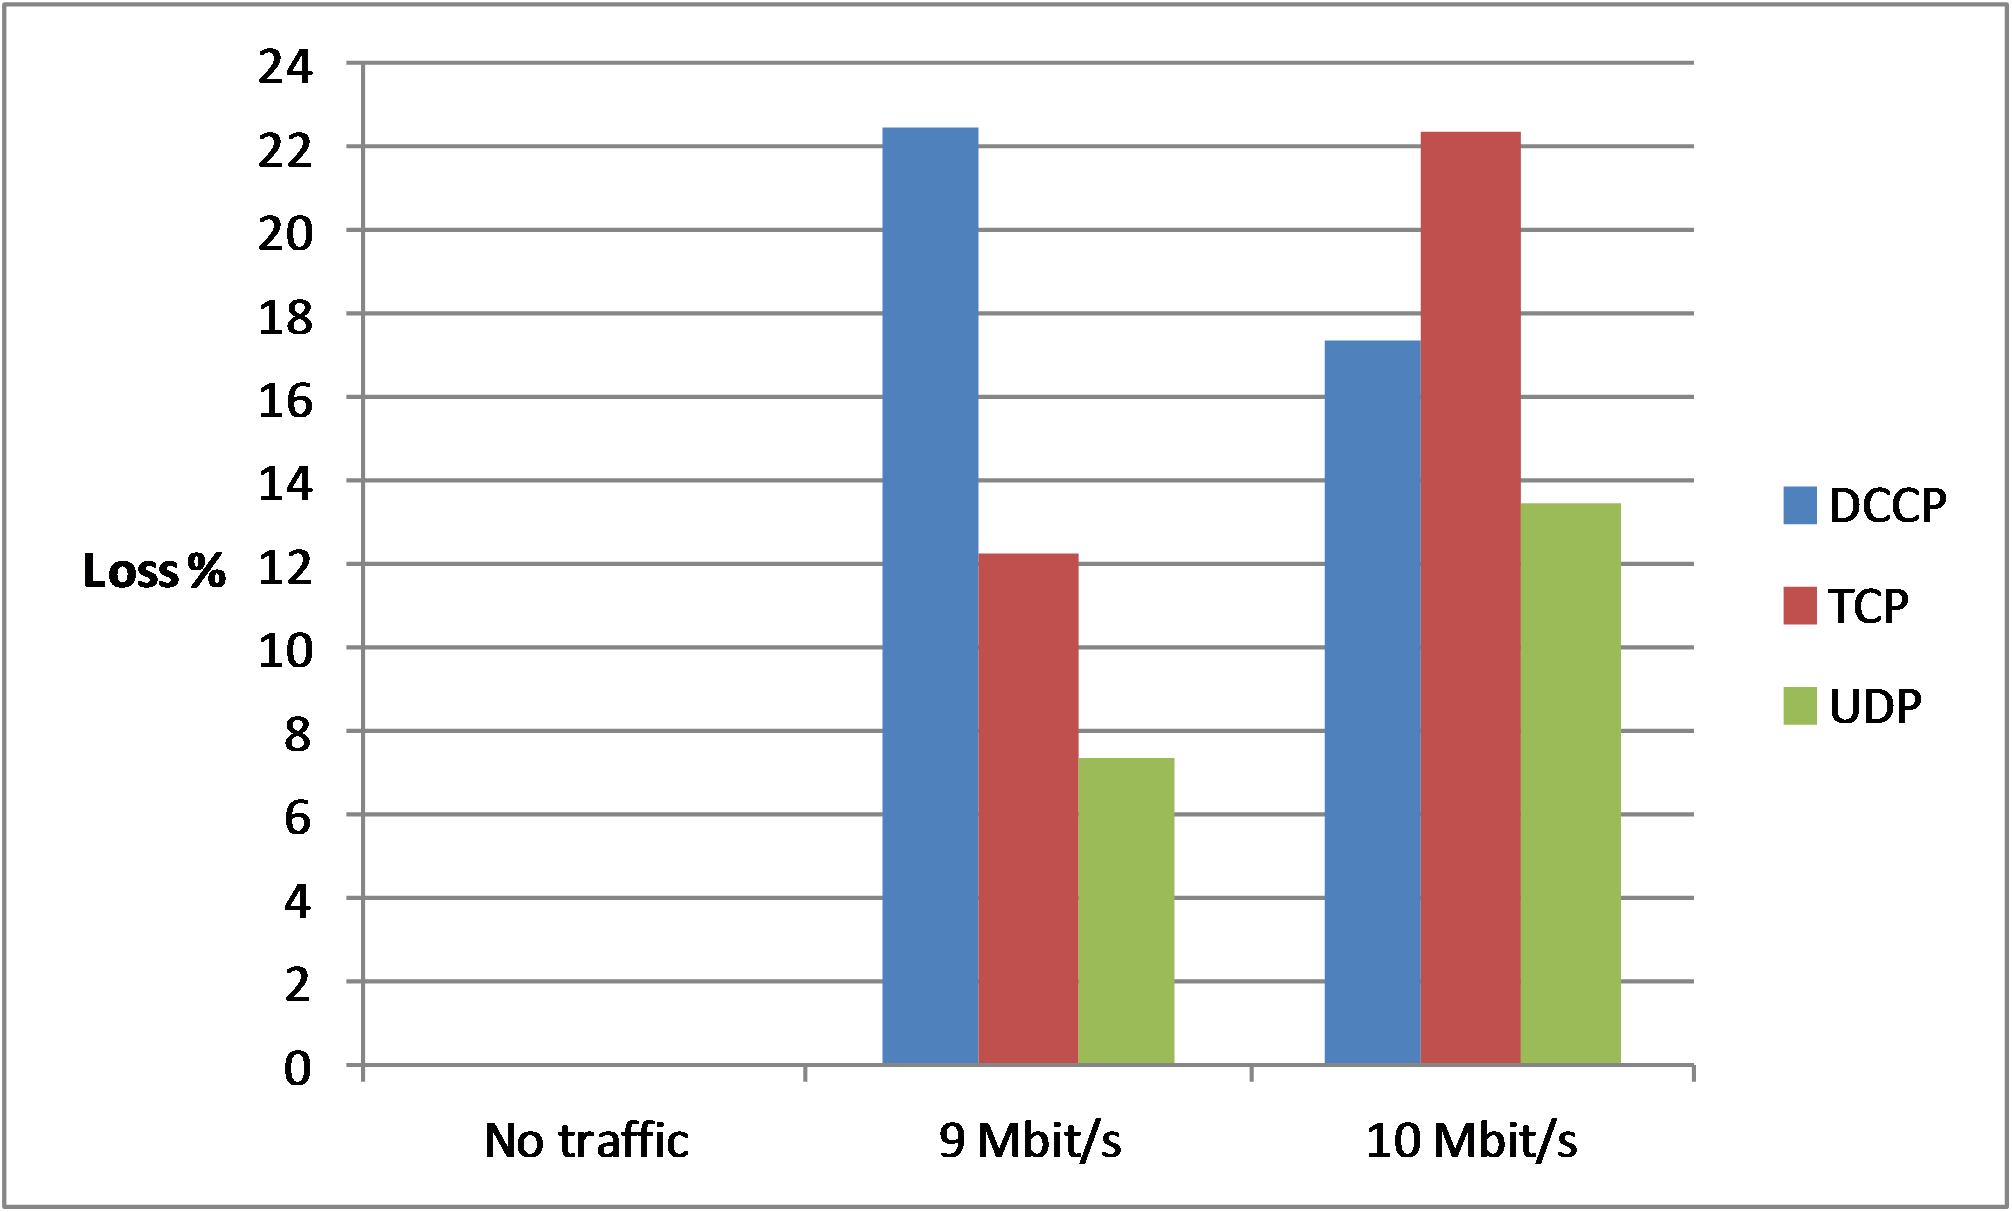
\includegraphics[width=0.45\textwidth]{pics/avg_losses}
   \caption{Average packet losses for each protocol.}
\label{fig:avg_losses}
\end{figure}

\begin{figure}[h]
   \centering
      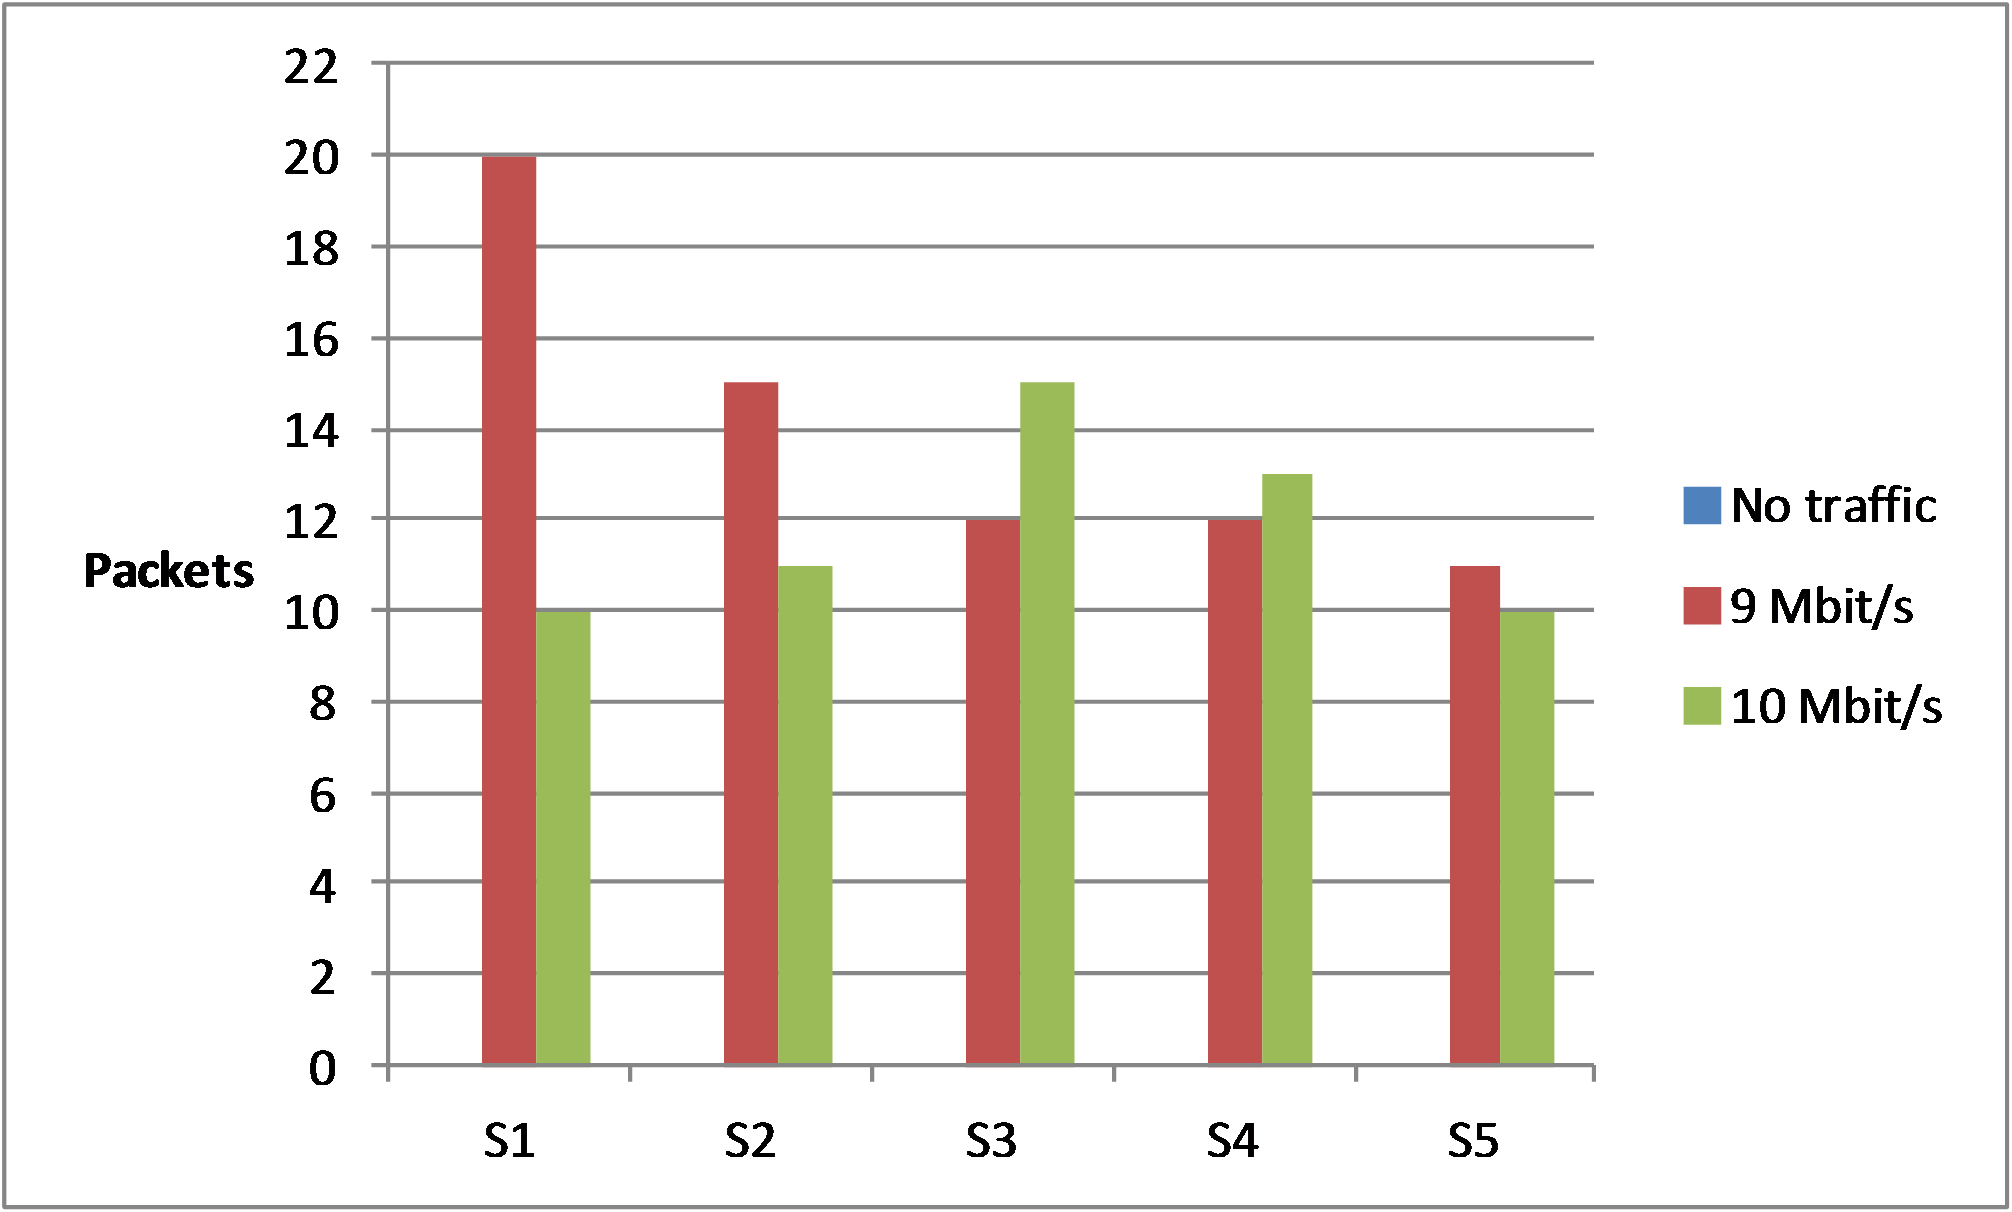
\includegraphics[width=0.45\textwidth]{pics/dccp_losses}
   \caption{Packets lost for all DCCP runs.}
\label{fig:dccp_losses}
\end{figure}

\begin{figure}[h]
   \centering
      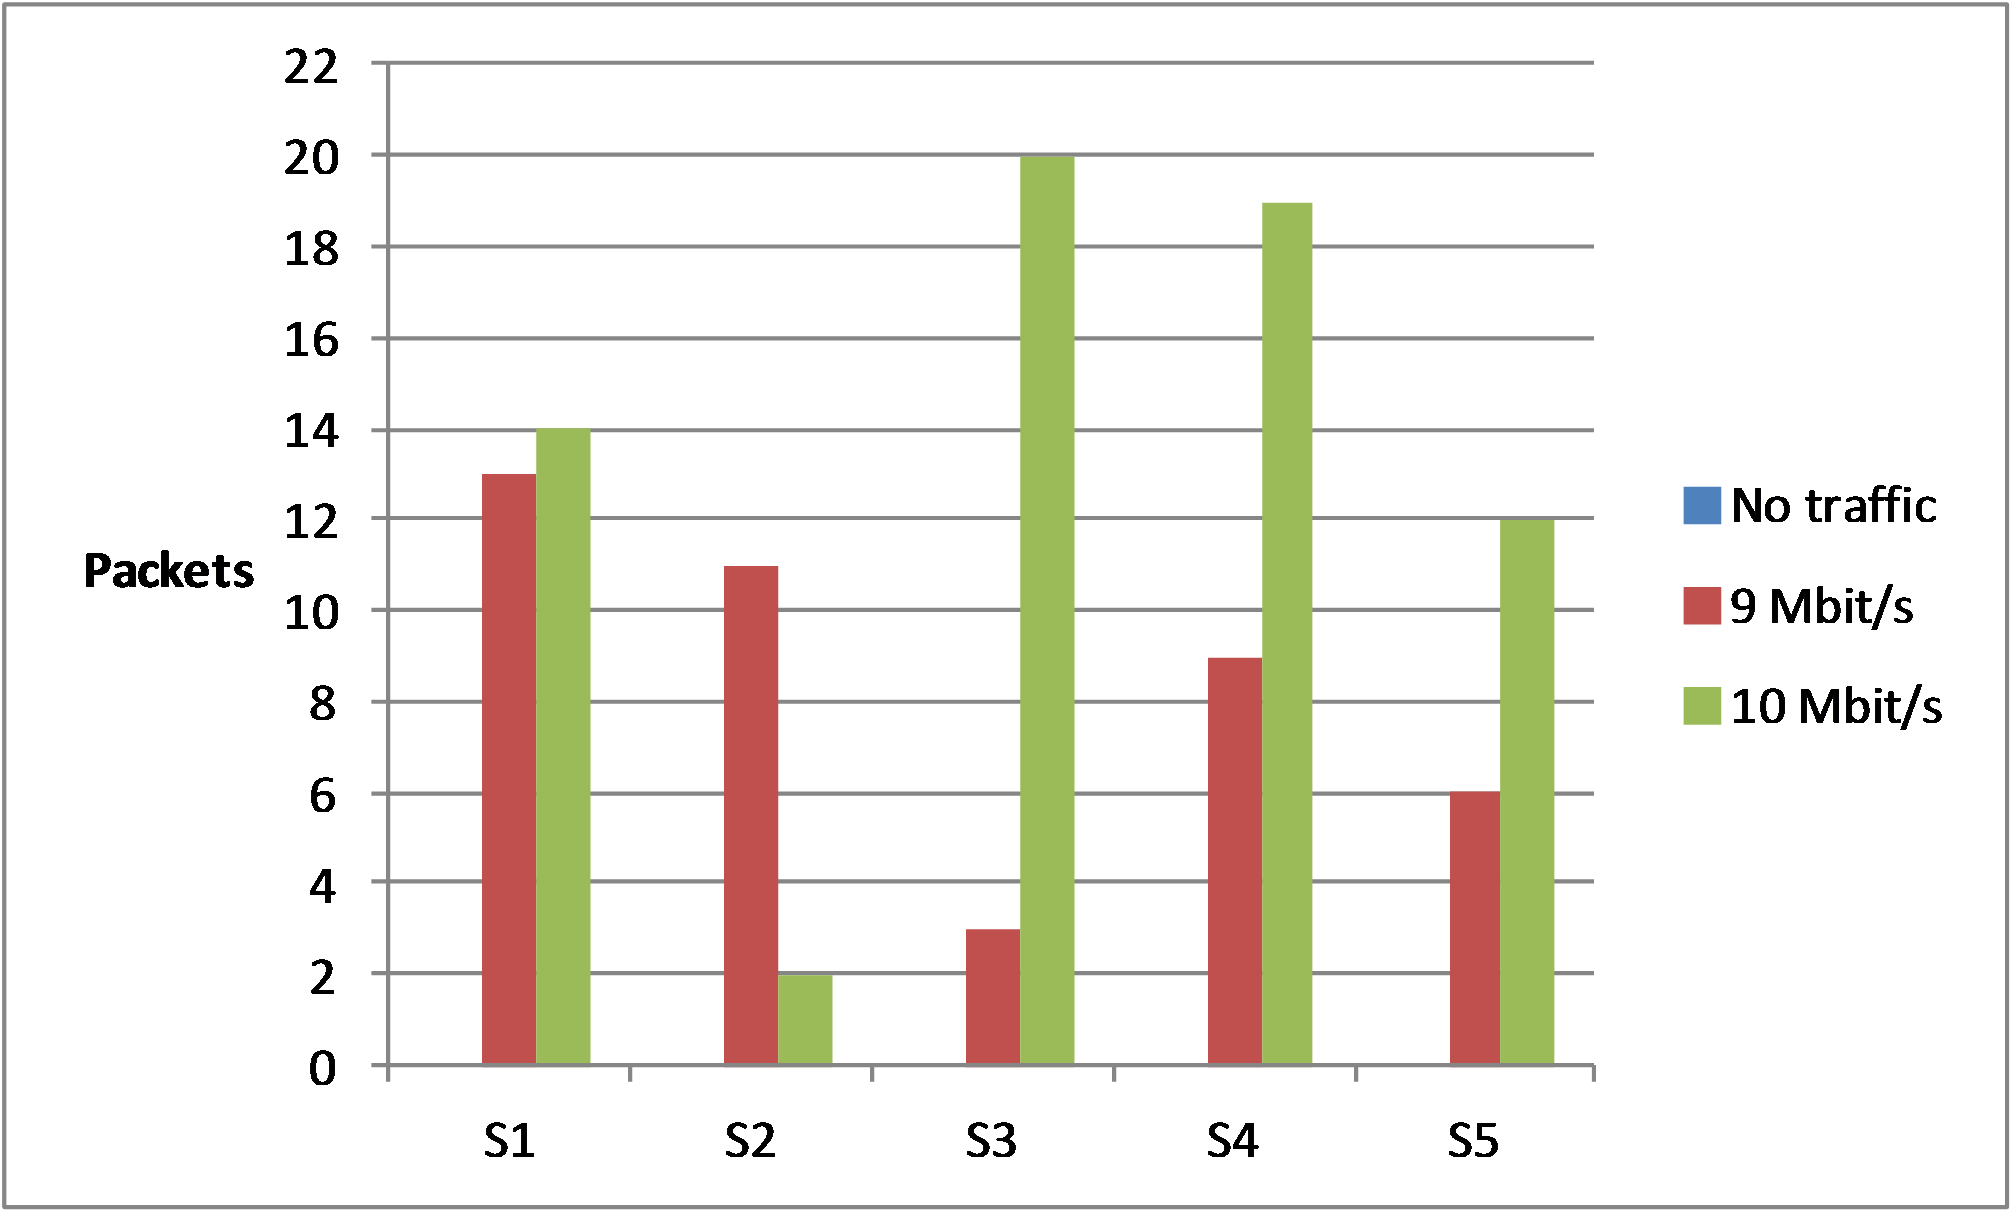
\includegraphics[width=0.45\textwidth]{pics/tcp_losses}
   \caption{Packets lost for all TCP runs.}
\label{fig:tcp_losses}
\end{figure}

\begin{figure}[h]
   \centering
      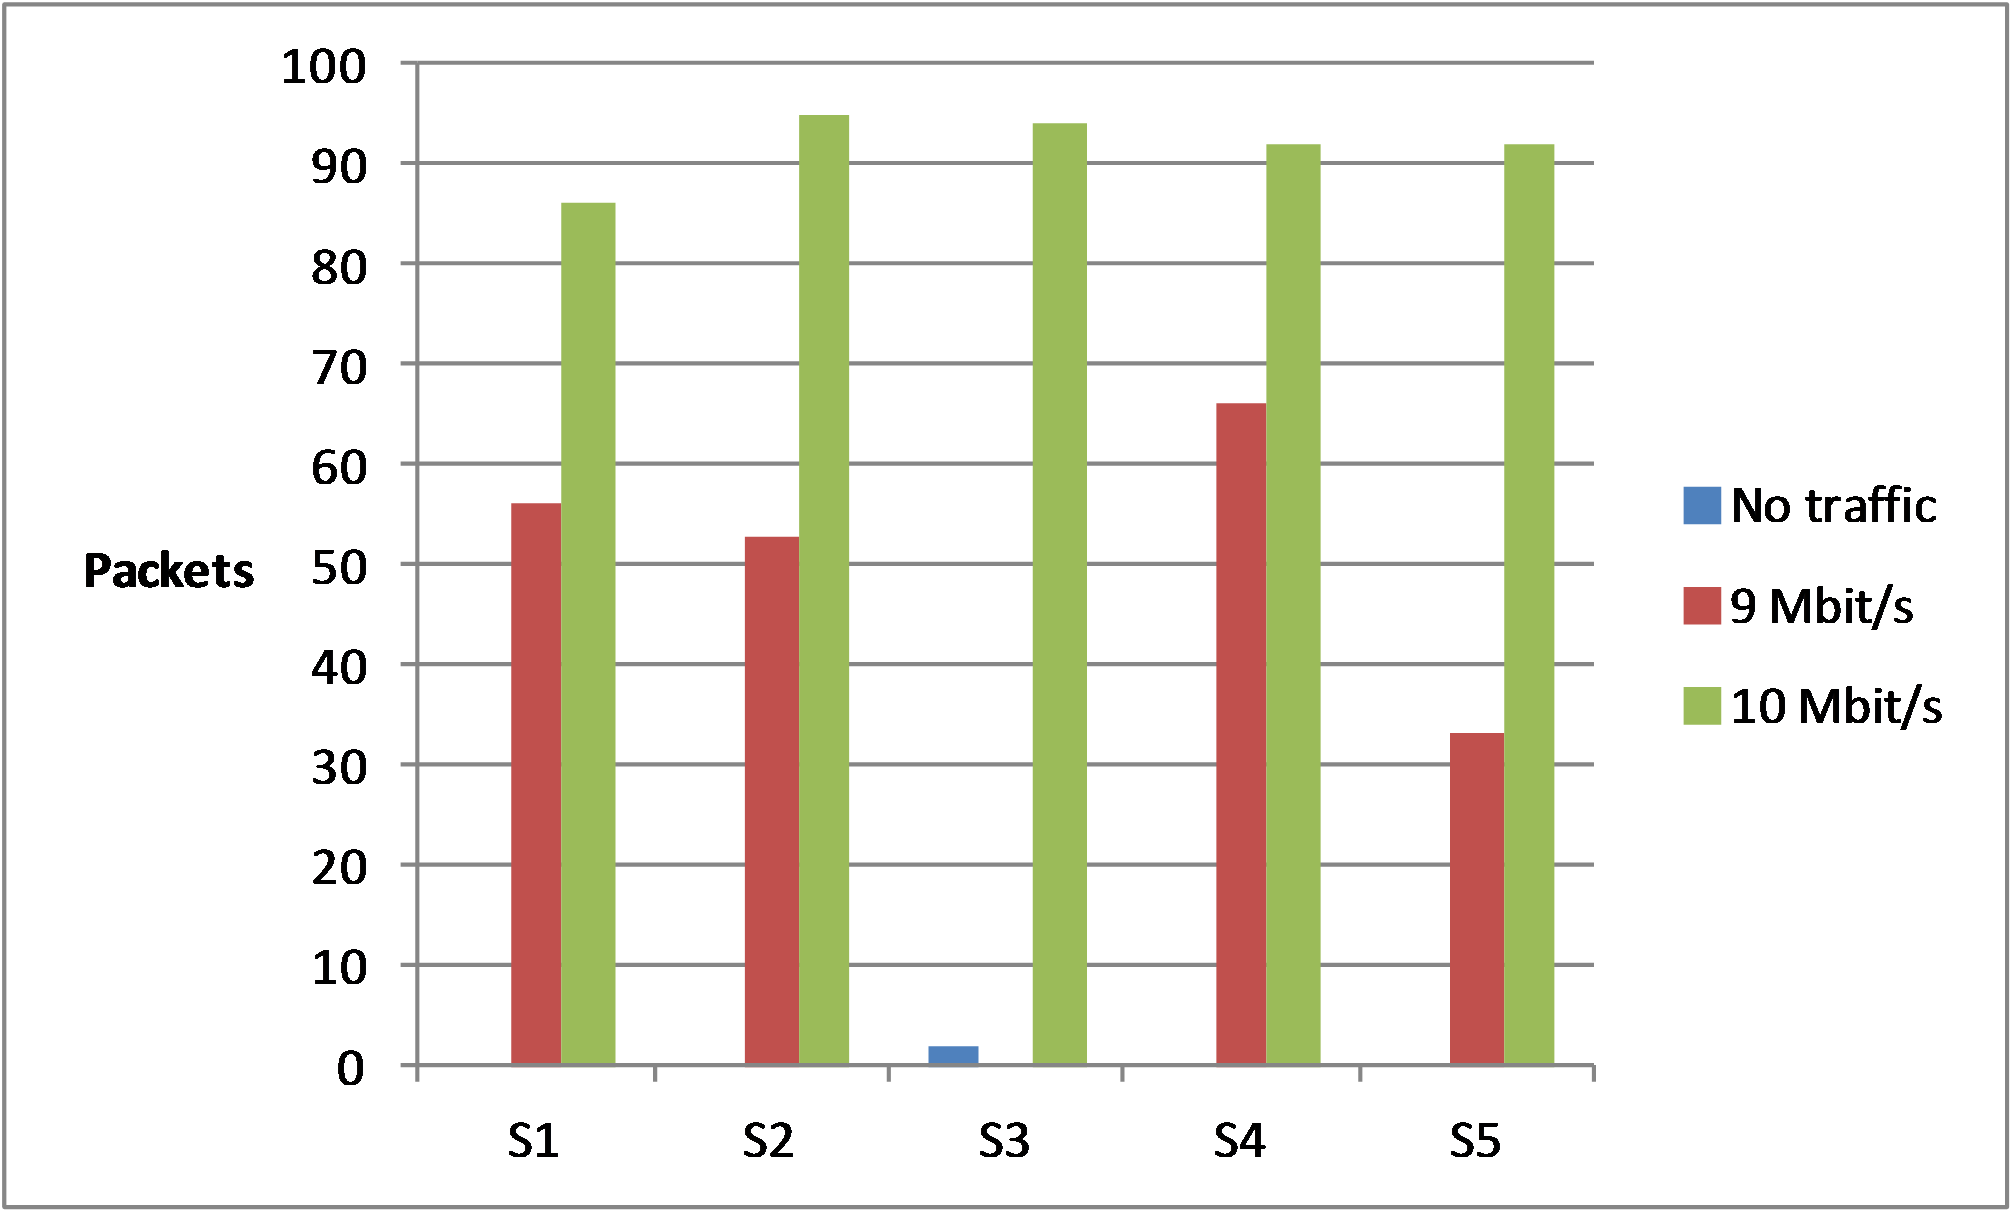
\includegraphics[width=0.45\textwidth]{pics/udp_losses}
   \caption{Packets lost for all UDP runs.}
\label{fig:udp_losses}
\end{figure}

Our experiments also allowed us to observe how each protocol throttled its
sending rate in response to increasing network congestion. Figures
~\ref{fig:dccp_sent},~\ref{fig:tcp_sent}, and~\ref{fig:udp_sent} give our
measurements.\\

As expected, DCCP and TCP transmit significantly fewer packets when congestion
is severe, but UDP continues to send approximately the same volume of packets
regardless of network conditions. In particular, TCP's behavior is extremely
regular, with each run producing very similar results. On the other hand, DCCP
demonstrated substantial variability in our tests with no background traffic.
Session 5 in particular showed a transmission rate comparable to that observed
during high congestion. However, since there was no other competing traffic on
the network during these tests, we do not believe the DCCP protocol itself is
responsible for this behavior. Rather, we believe the host laptop's operating
system or a bug in our chat program may have sometimes caused a lower packet
volume.

\begin{figure}[h]
   \centering
      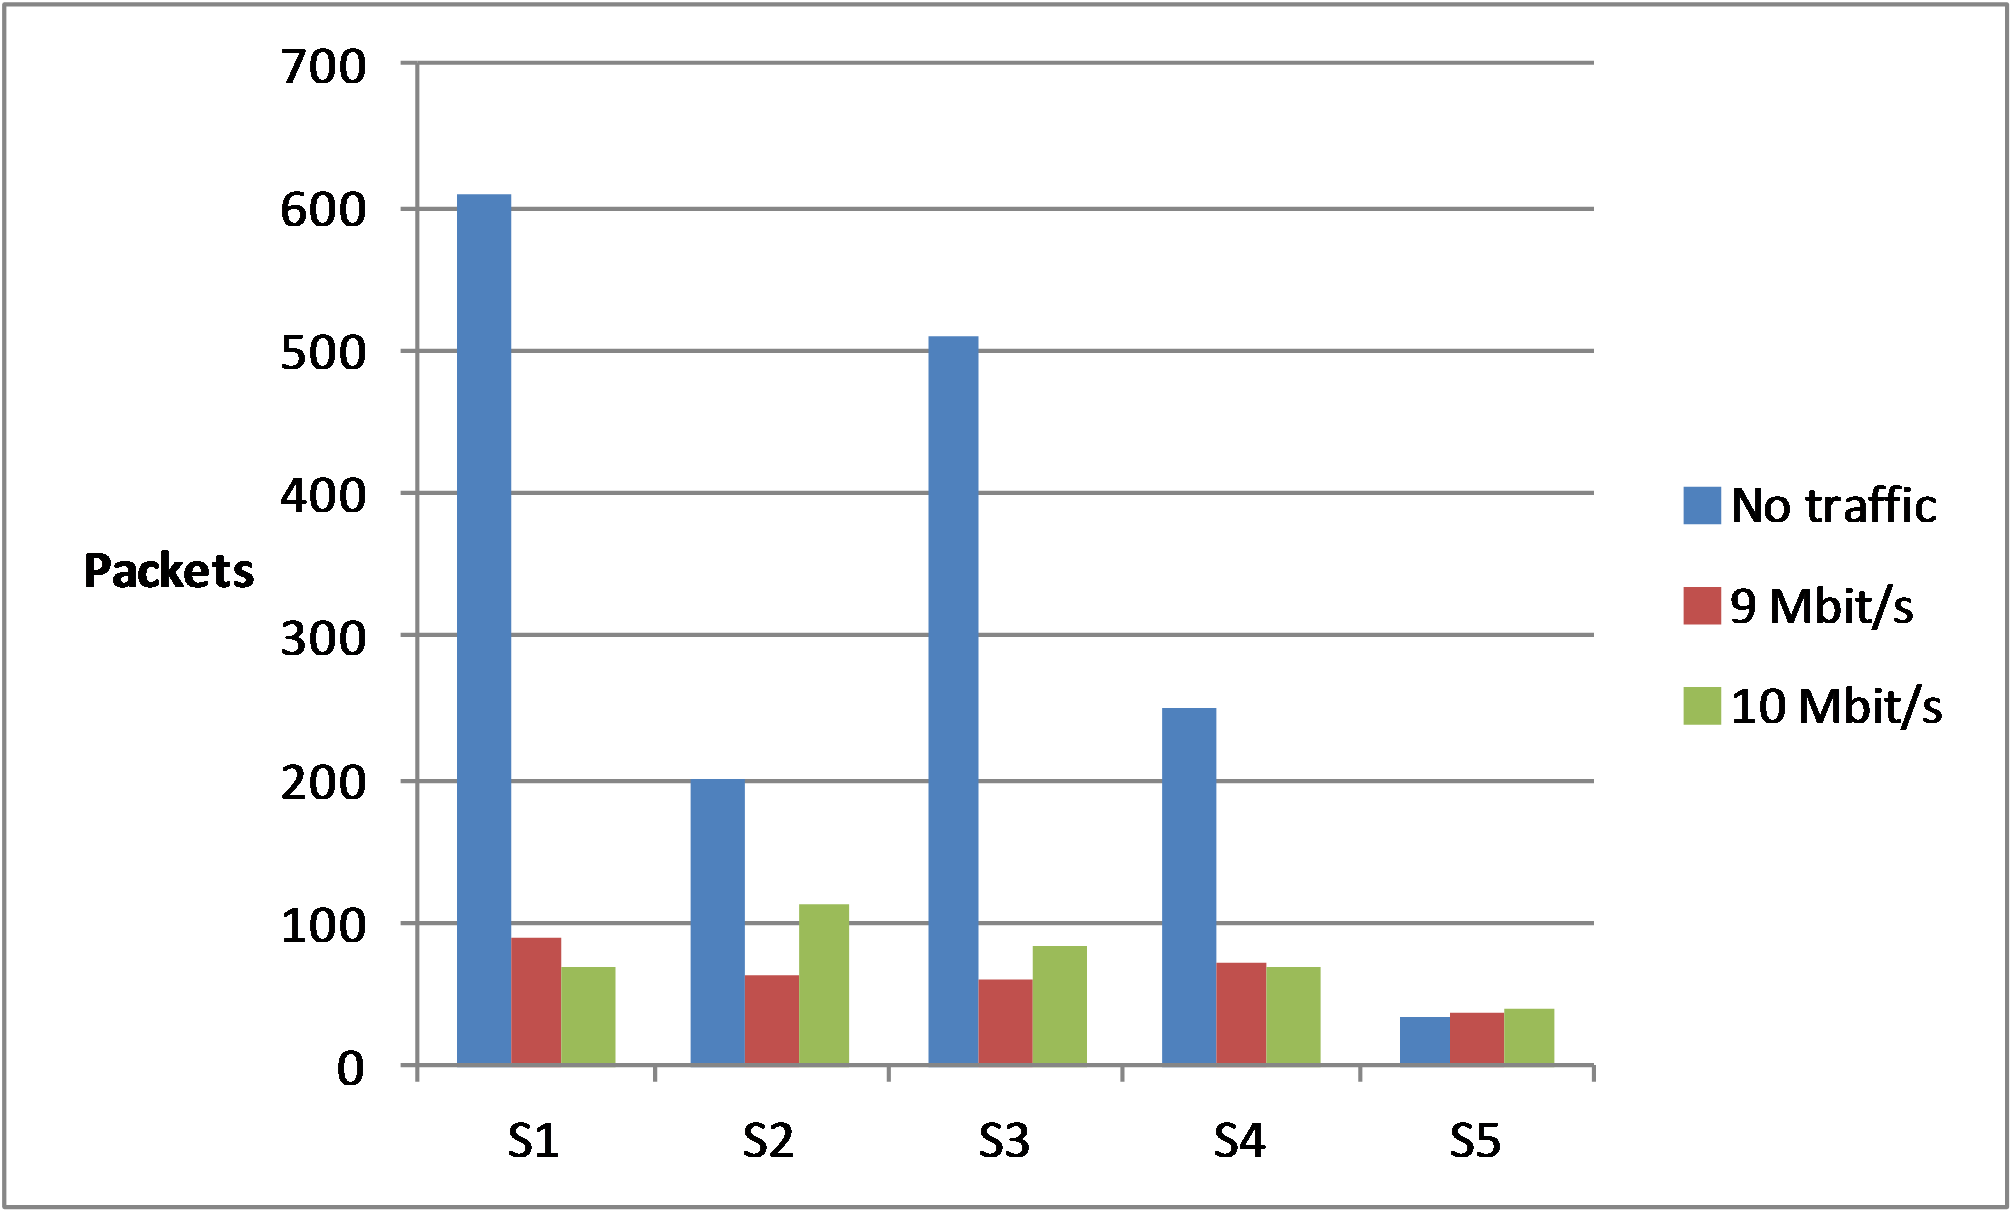
\includegraphics[width=0.45\textwidth]{pics/dccp_sent}
   \caption{Packets sent during all DCCP tests.}
\label{fig:dccp_sent}
\end{figure}

\begin{figure}[h]
   \centering
      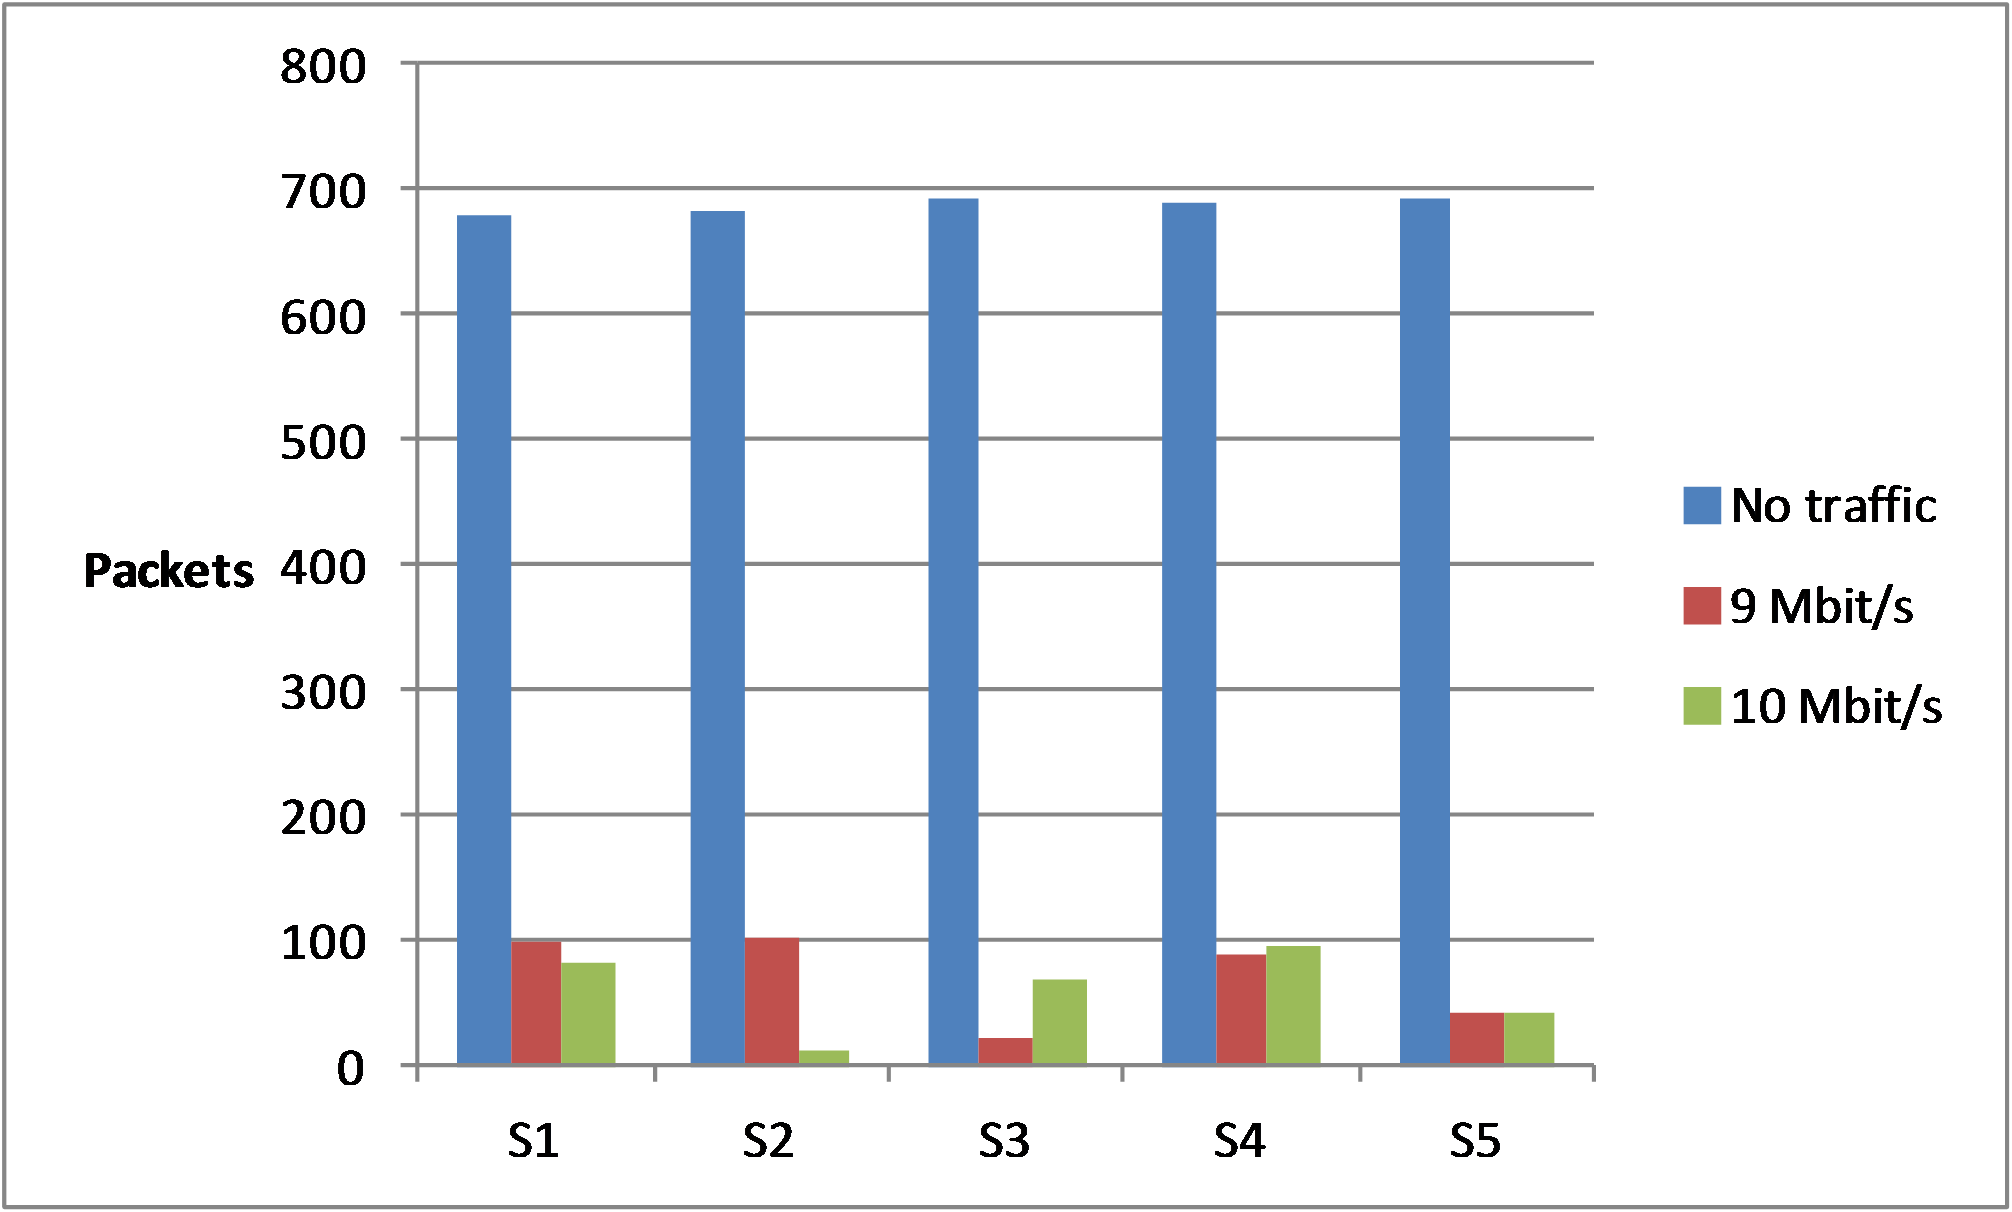
\includegraphics[width=0.45\textwidth]{pics/tcp_sent}
   \caption{Packets sent during all TCP tests.}
\label{fig:tcp_sent}
\end{figure}

\begin{figure}[h]
   \centering
      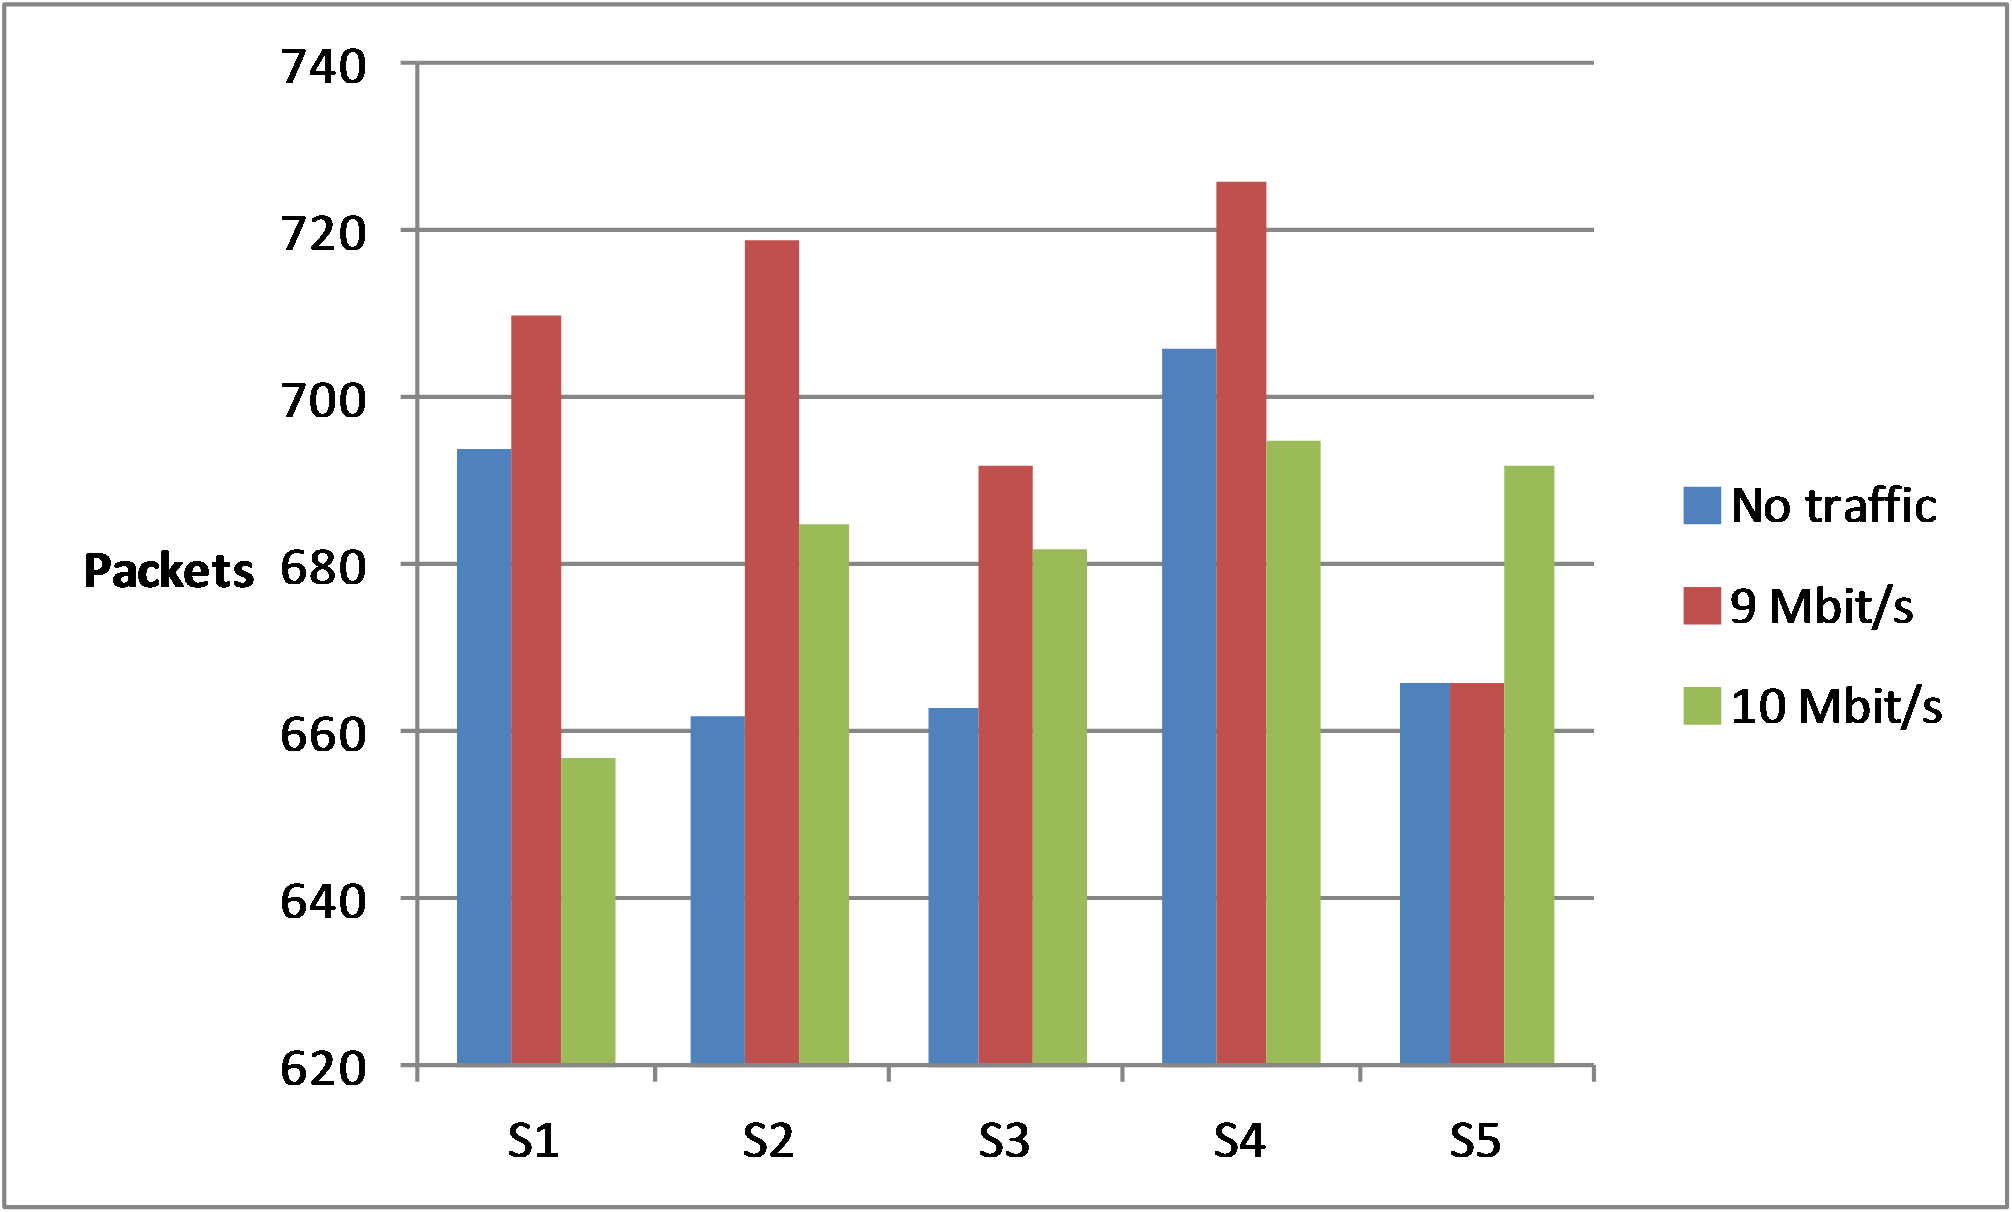
\includegraphics[width=0.45\textwidth]{pics/udp_sent}
   \caption{Packets sent during all UDP tests.}
\label{fig:udp_sent}
\end{figure}

\subsubsection{Jitter}

This section gives our jitter measurements for each protocol at each of our
three background traffic levels. Each graph is a CDF of our aggregated jitter
measurements for each protocol and congestion level, convering all five
individual sessions.

\begin{figure}[h]
   \centering
      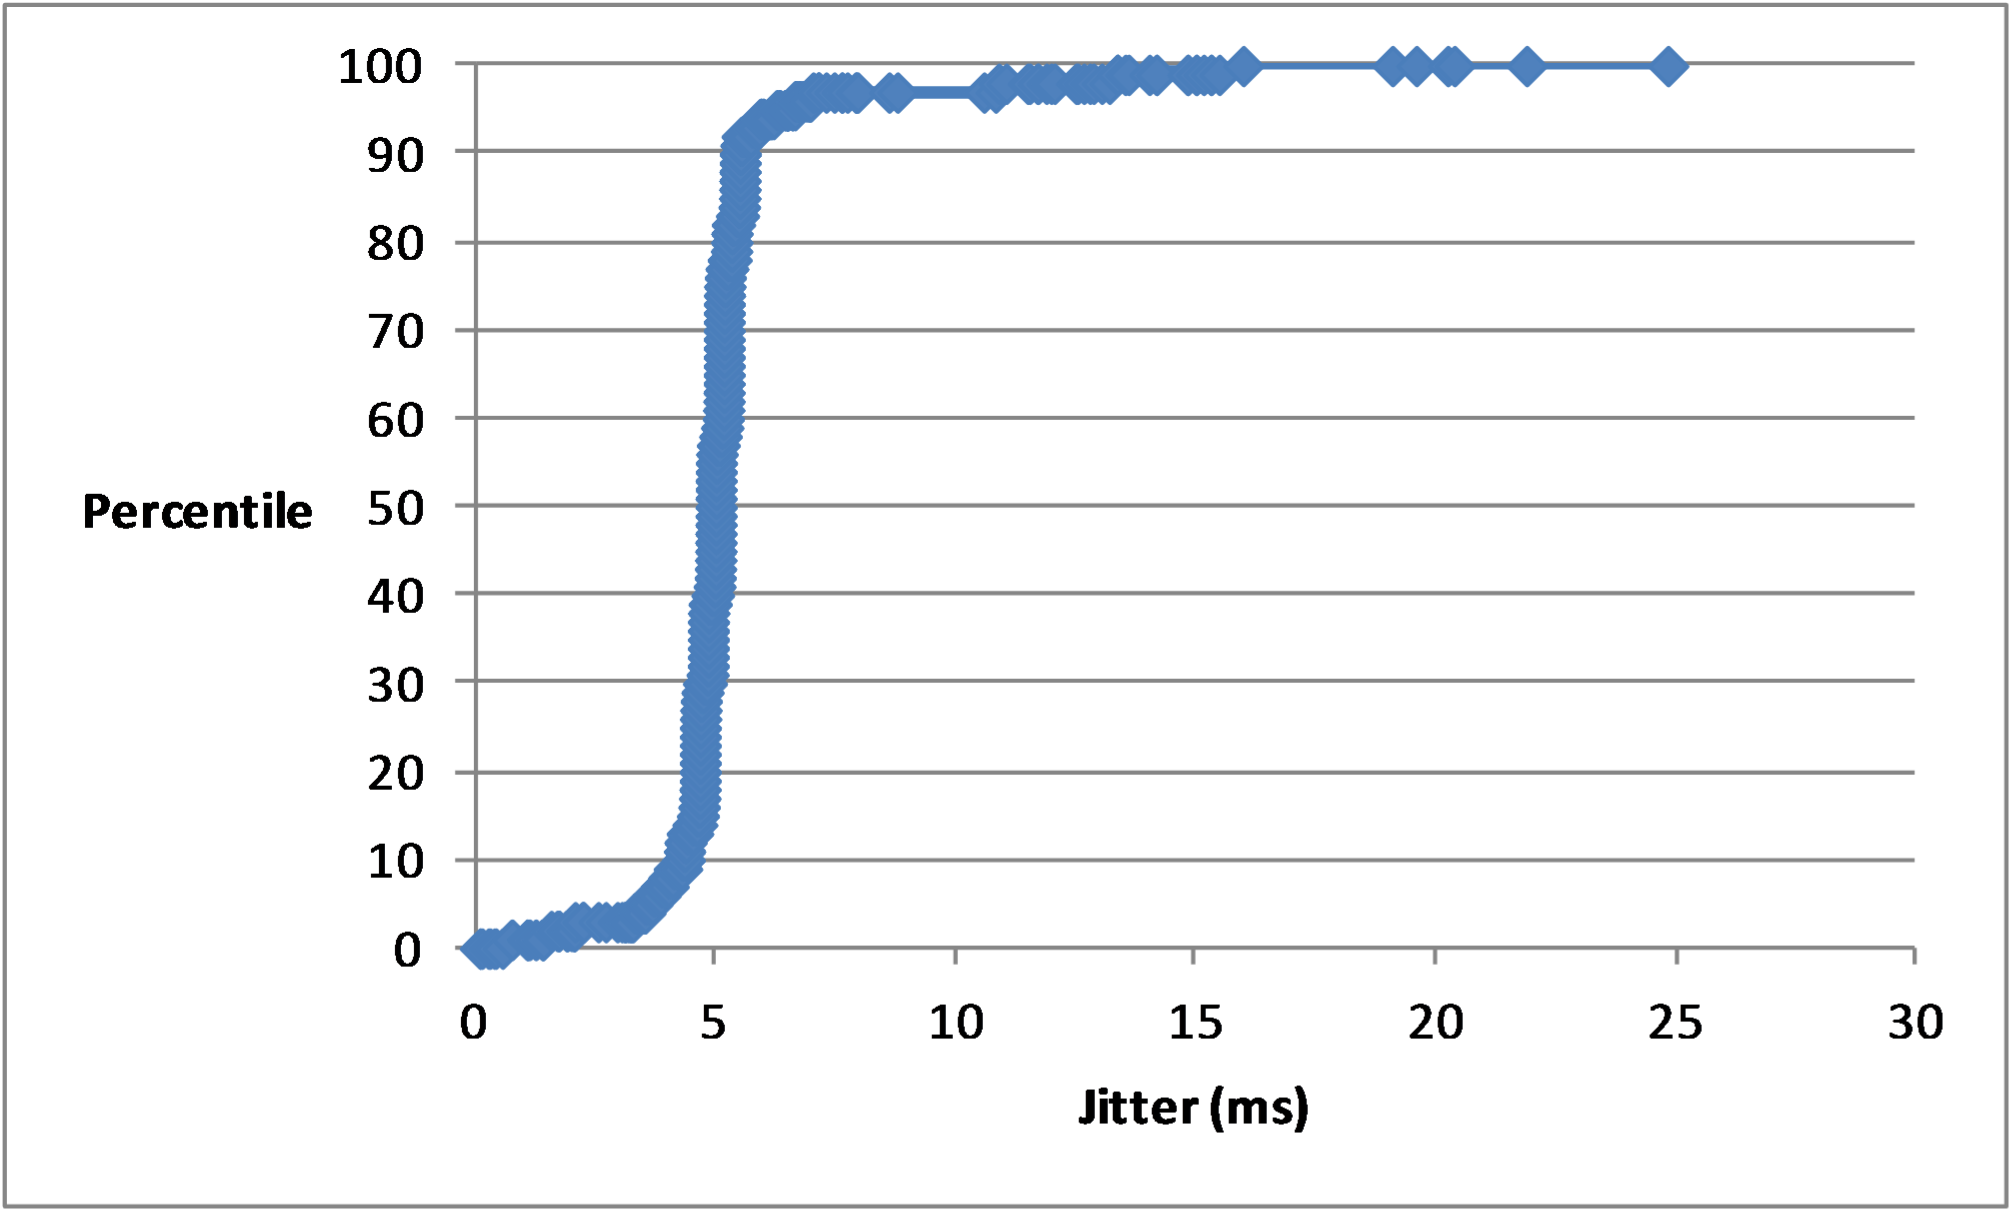
\includegraphics[width=0.45\textwidth]{pics/dccp_none_jitter}
   \caption{DCCP jitter CDF with no background traffic.}
\label{fig:dccp_none_jitter}
\end{figure}

\begin{figure}[h]
   \centering
      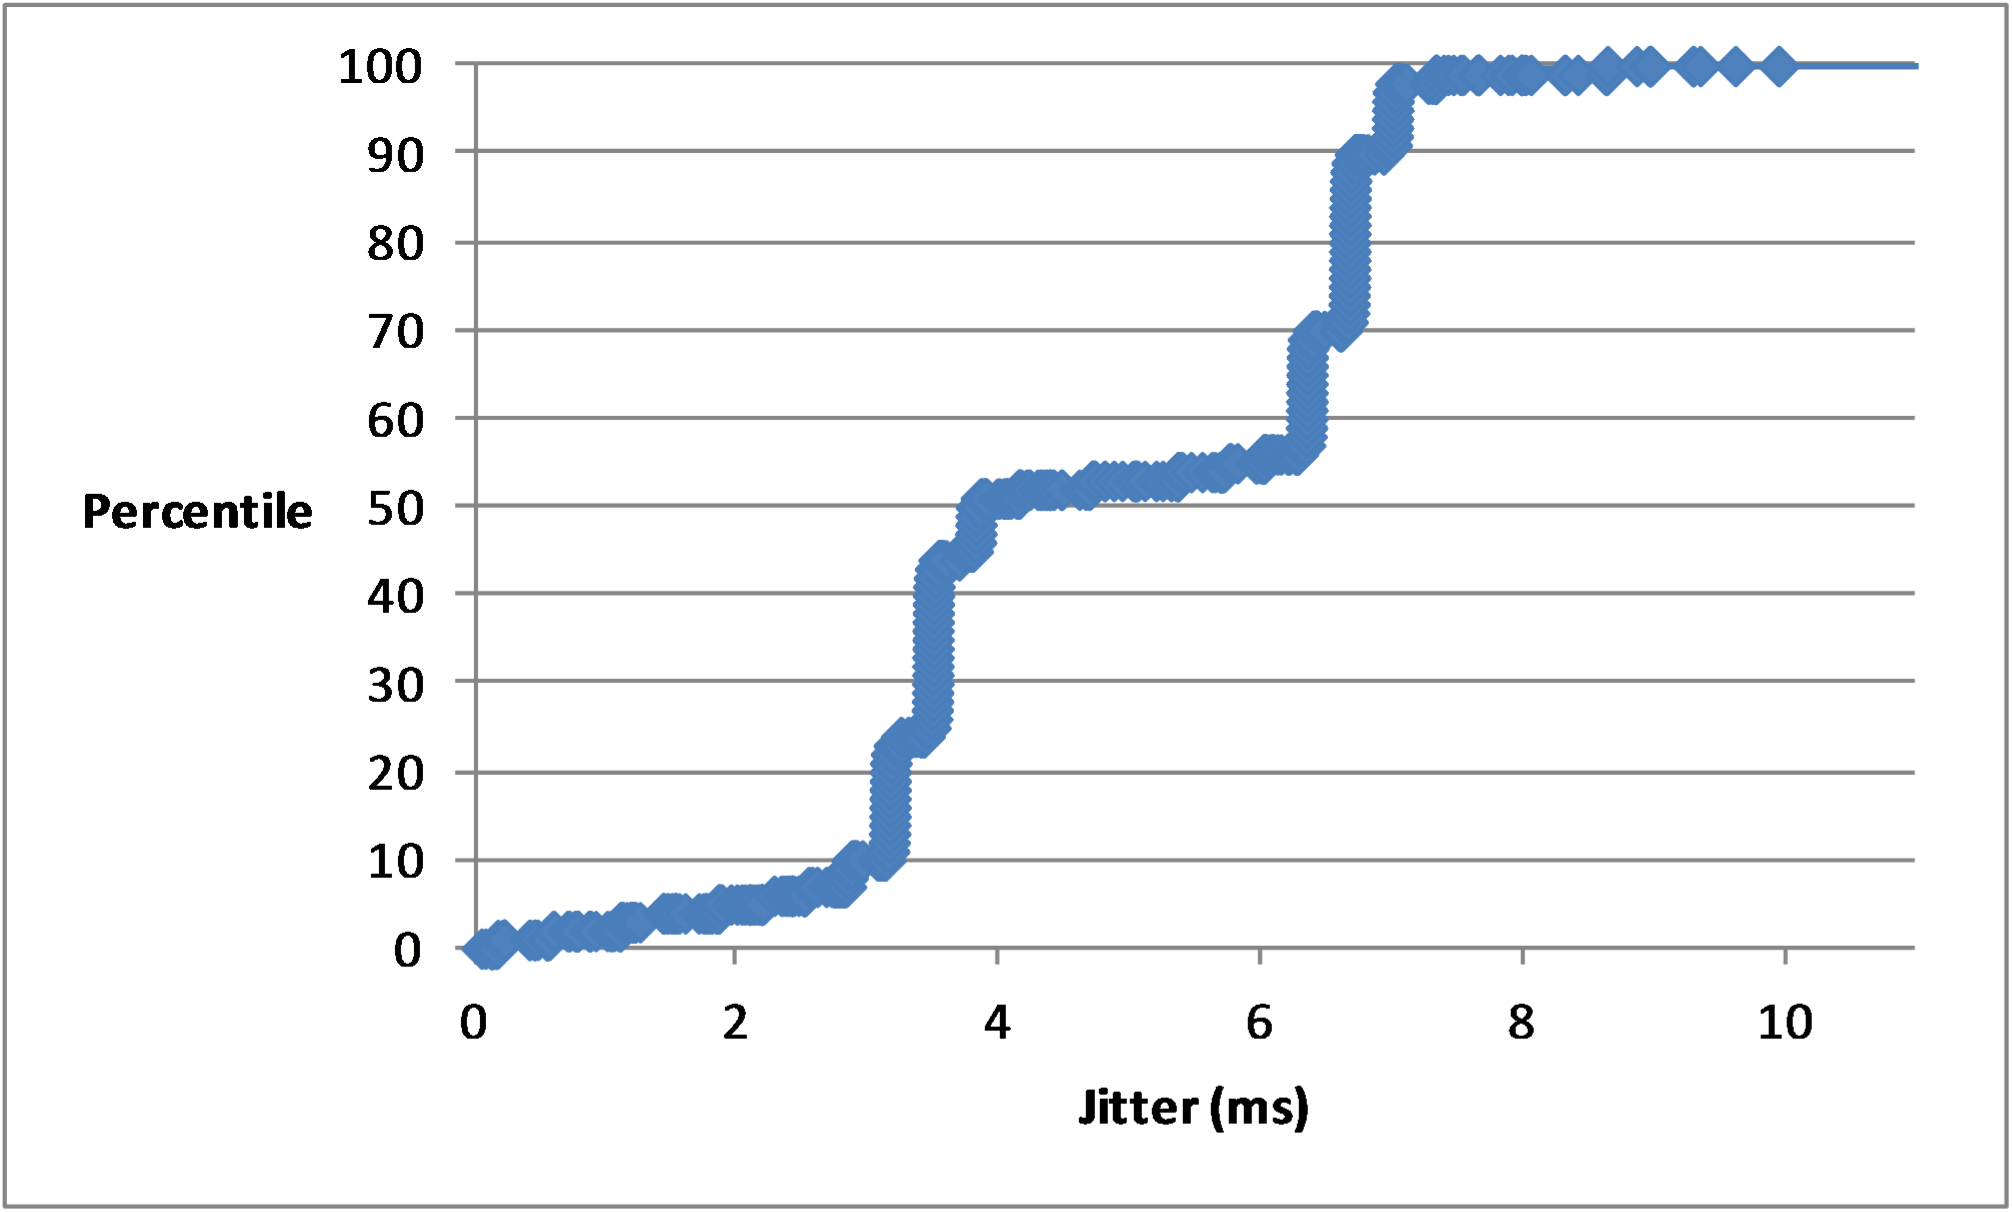
\includegraphics[width=0.45\textwidth]{pics/tcp_none_jitter}
   \caption{TCP jitter CDF with no background traffic.}
\label{fig:tcp_none_jitter}
\end{figure}

\begin{figure}[h]
   \centering
      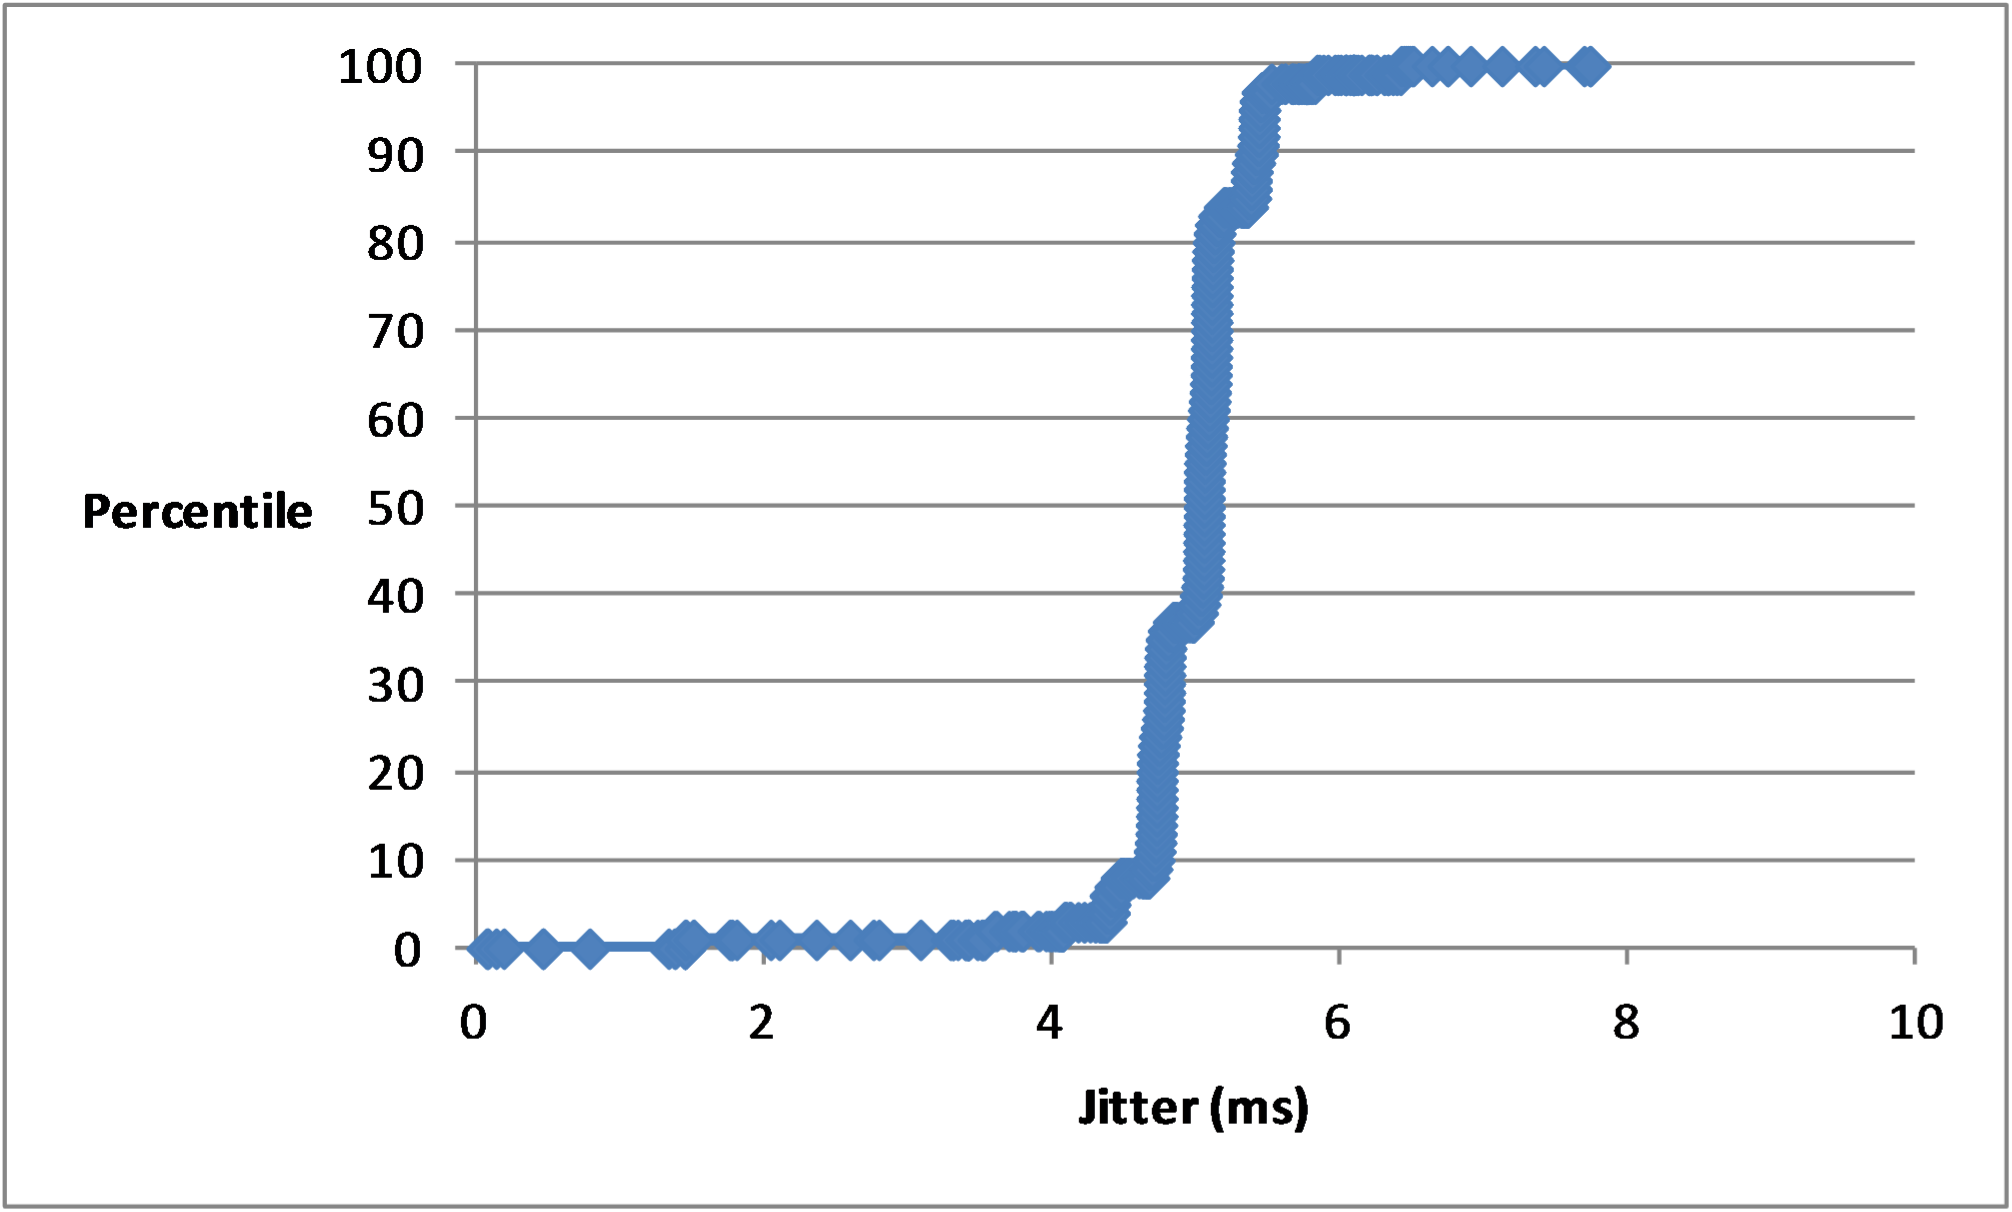
\includegraphics[width=0.45\textwidth]{pics/udp_none_jitter}
   \caption{UDP jitter CDF with no background traffic.}
\label{fig:udp_none_jitter}
\end{figure}

\begin{figure}[h]
   \centering
      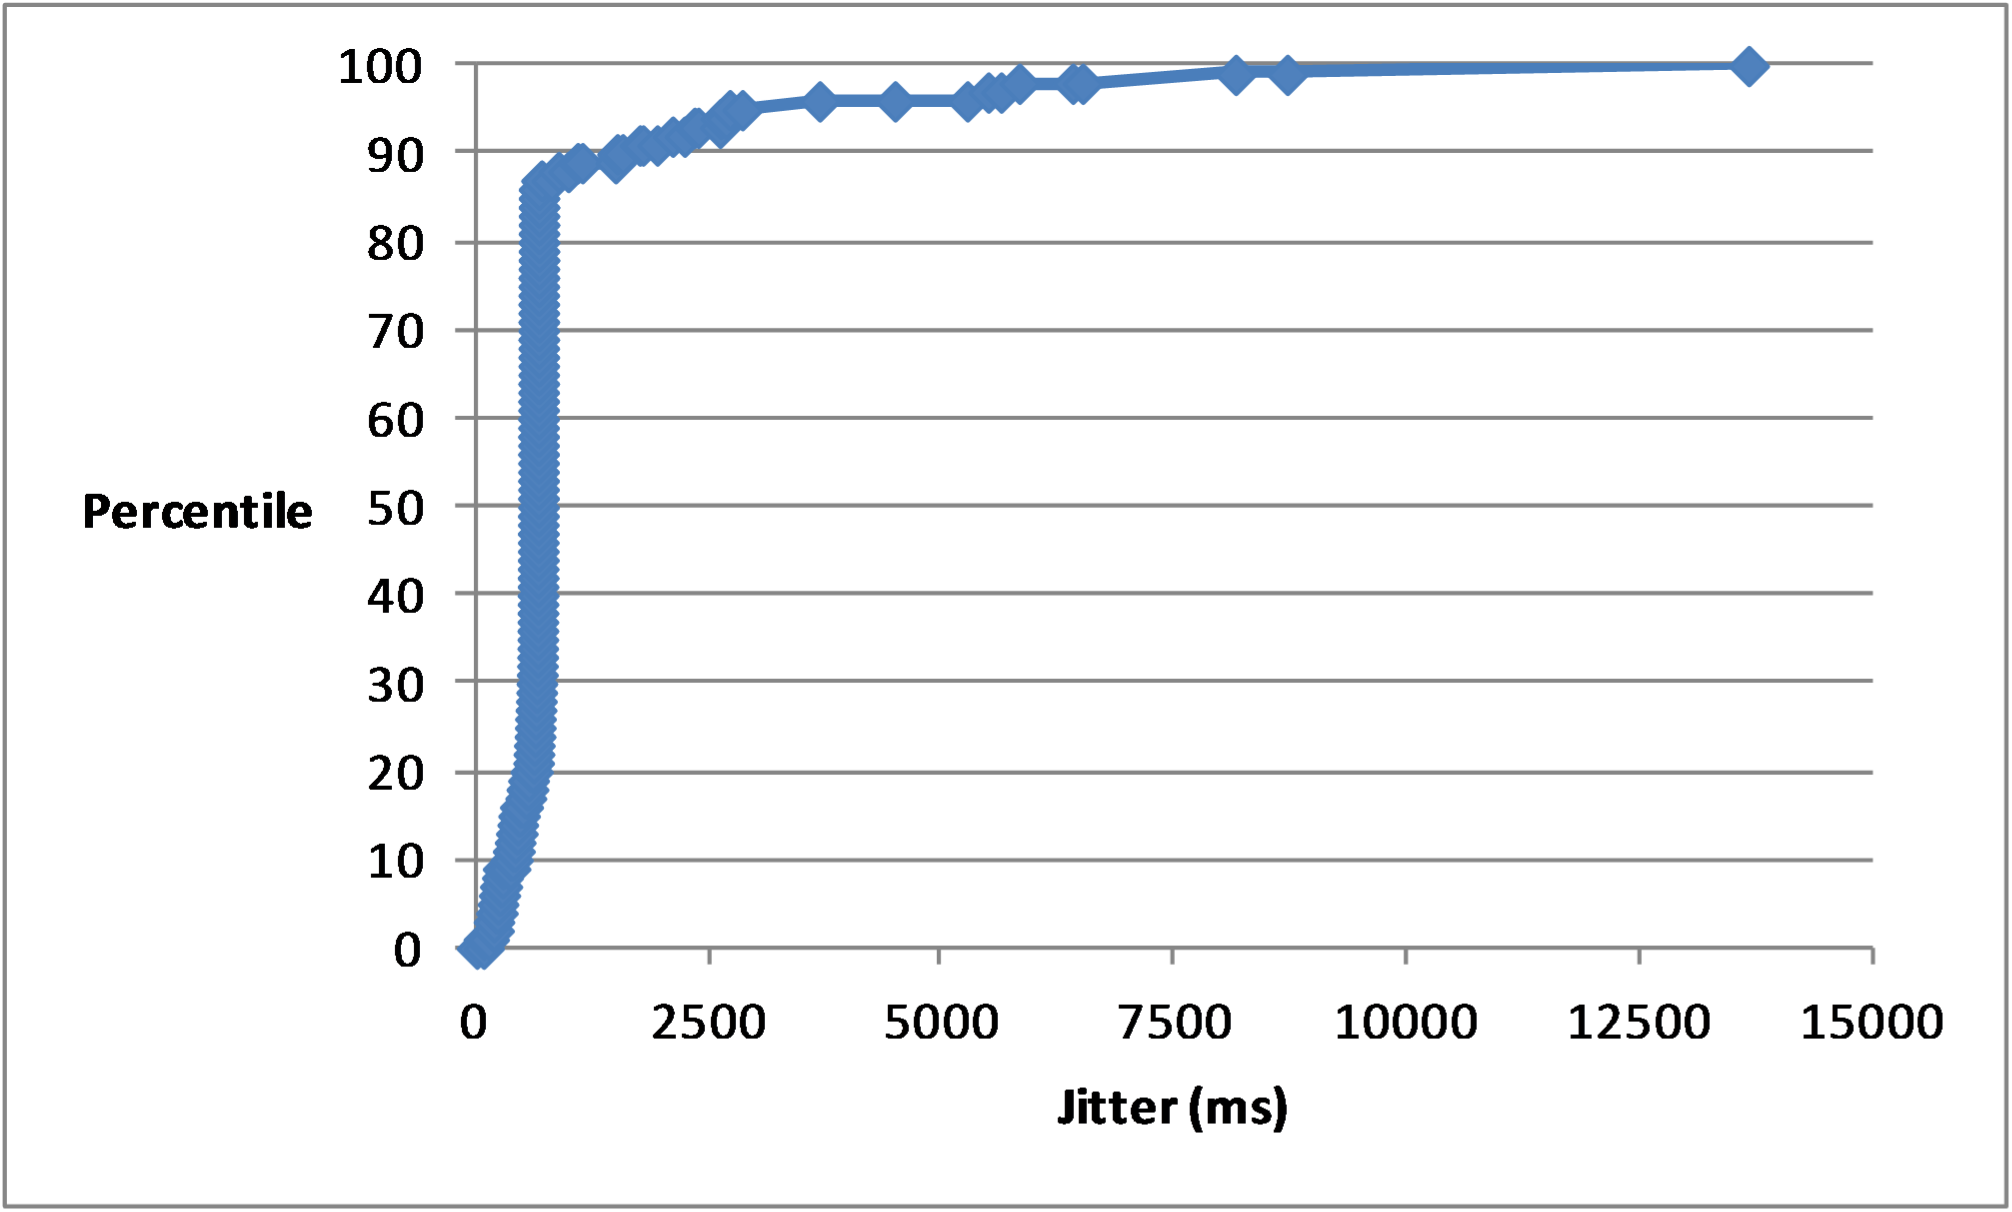
\includegraphics[width=0.45\textwidth]{pics/dccp_9_jitter_new}
   \caption{DCCP jitter CDF for 9 Mbit/s.}
\label{fig:dccp_9_jitter}
\end{figure}

\begin{figure}[h]
   \centering
      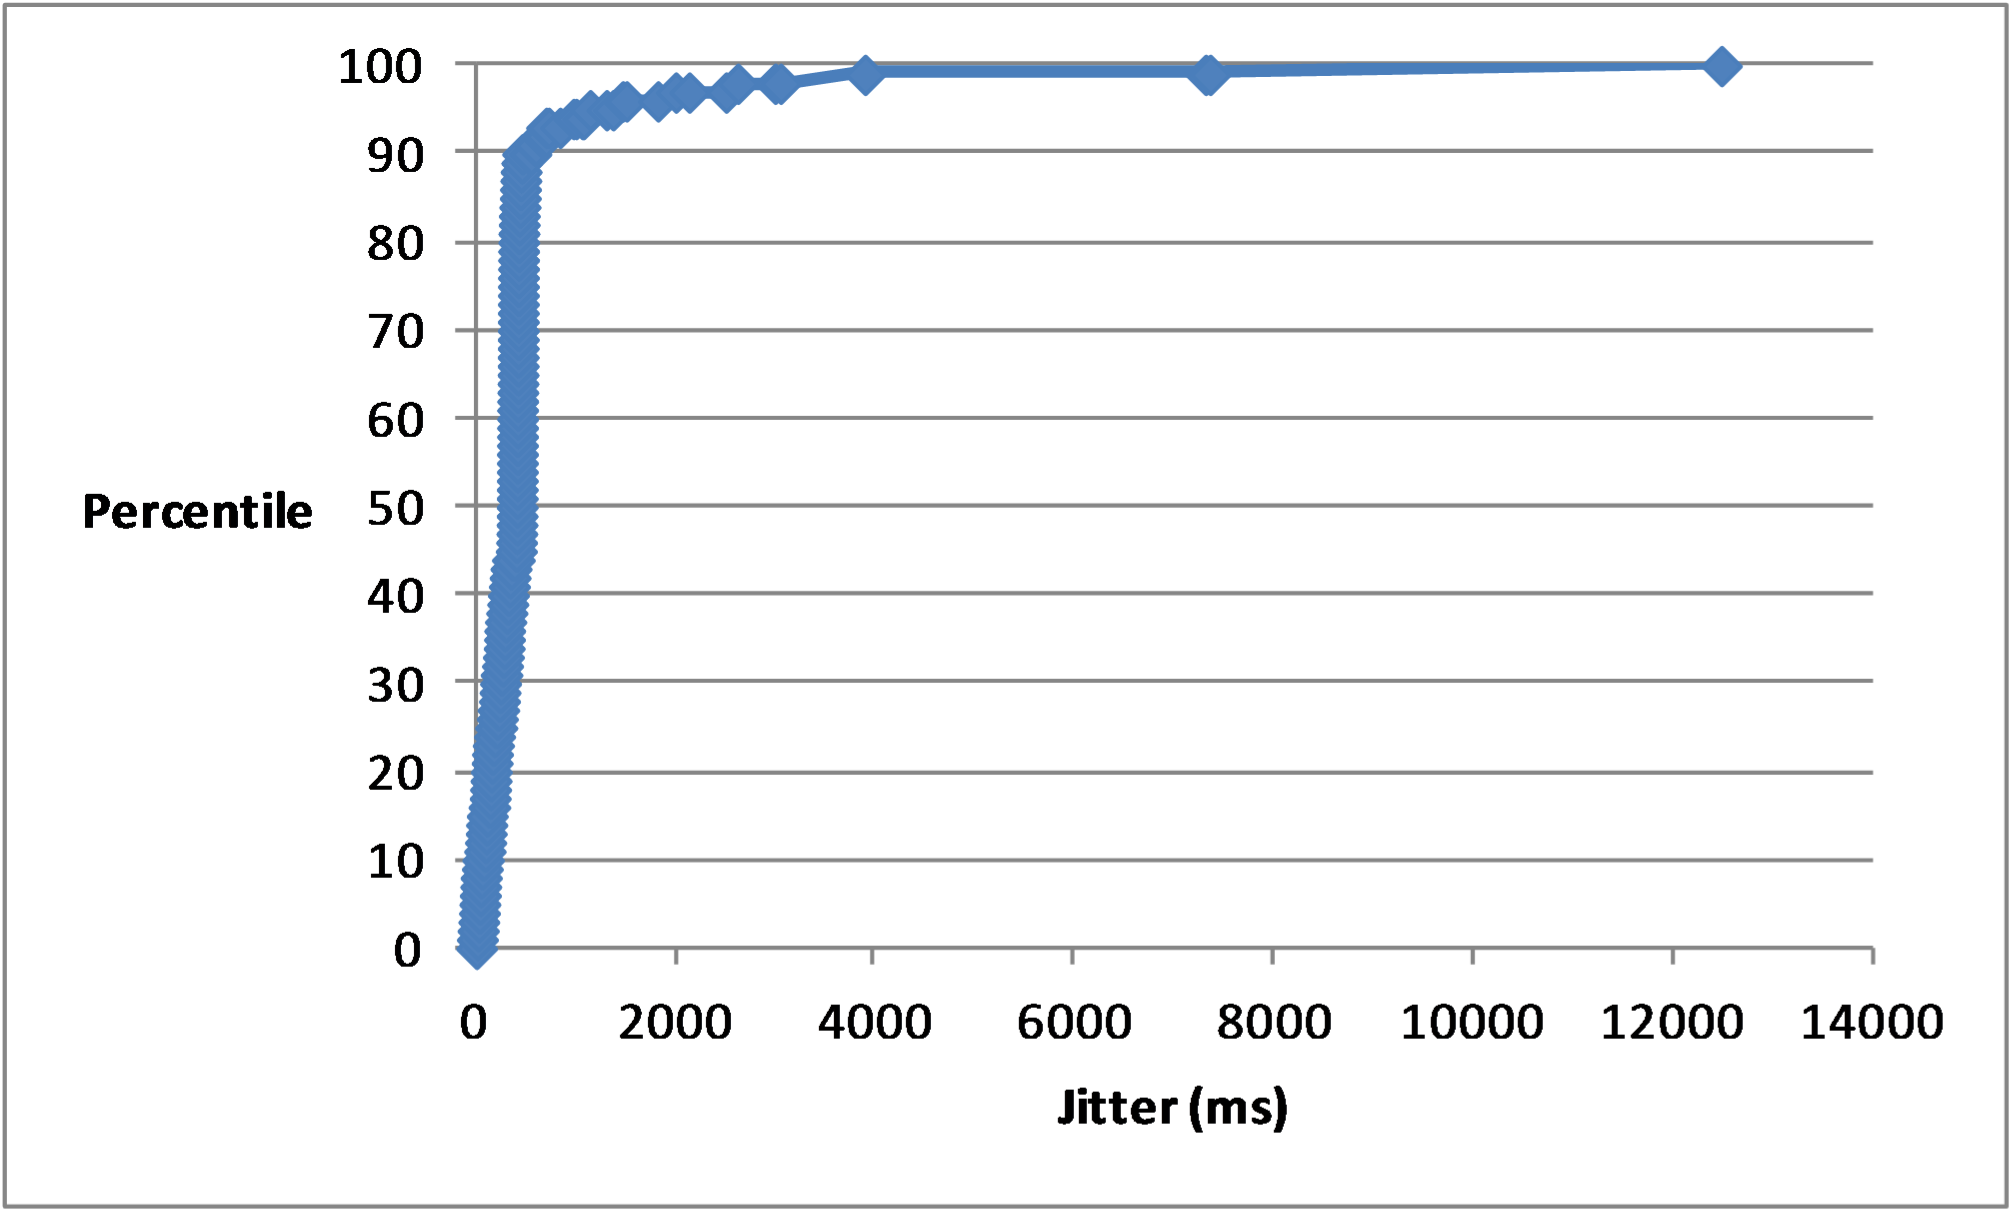
\includegraphics[width=0.45\textwidth]{pics/tcp_9_jitter}
   \caption{TCP jitter CDF for 9 Mbit/s.}
\label{fig:tcp_9_jitter}
\end{figure}

\begin{figure}[h]
   \centering
      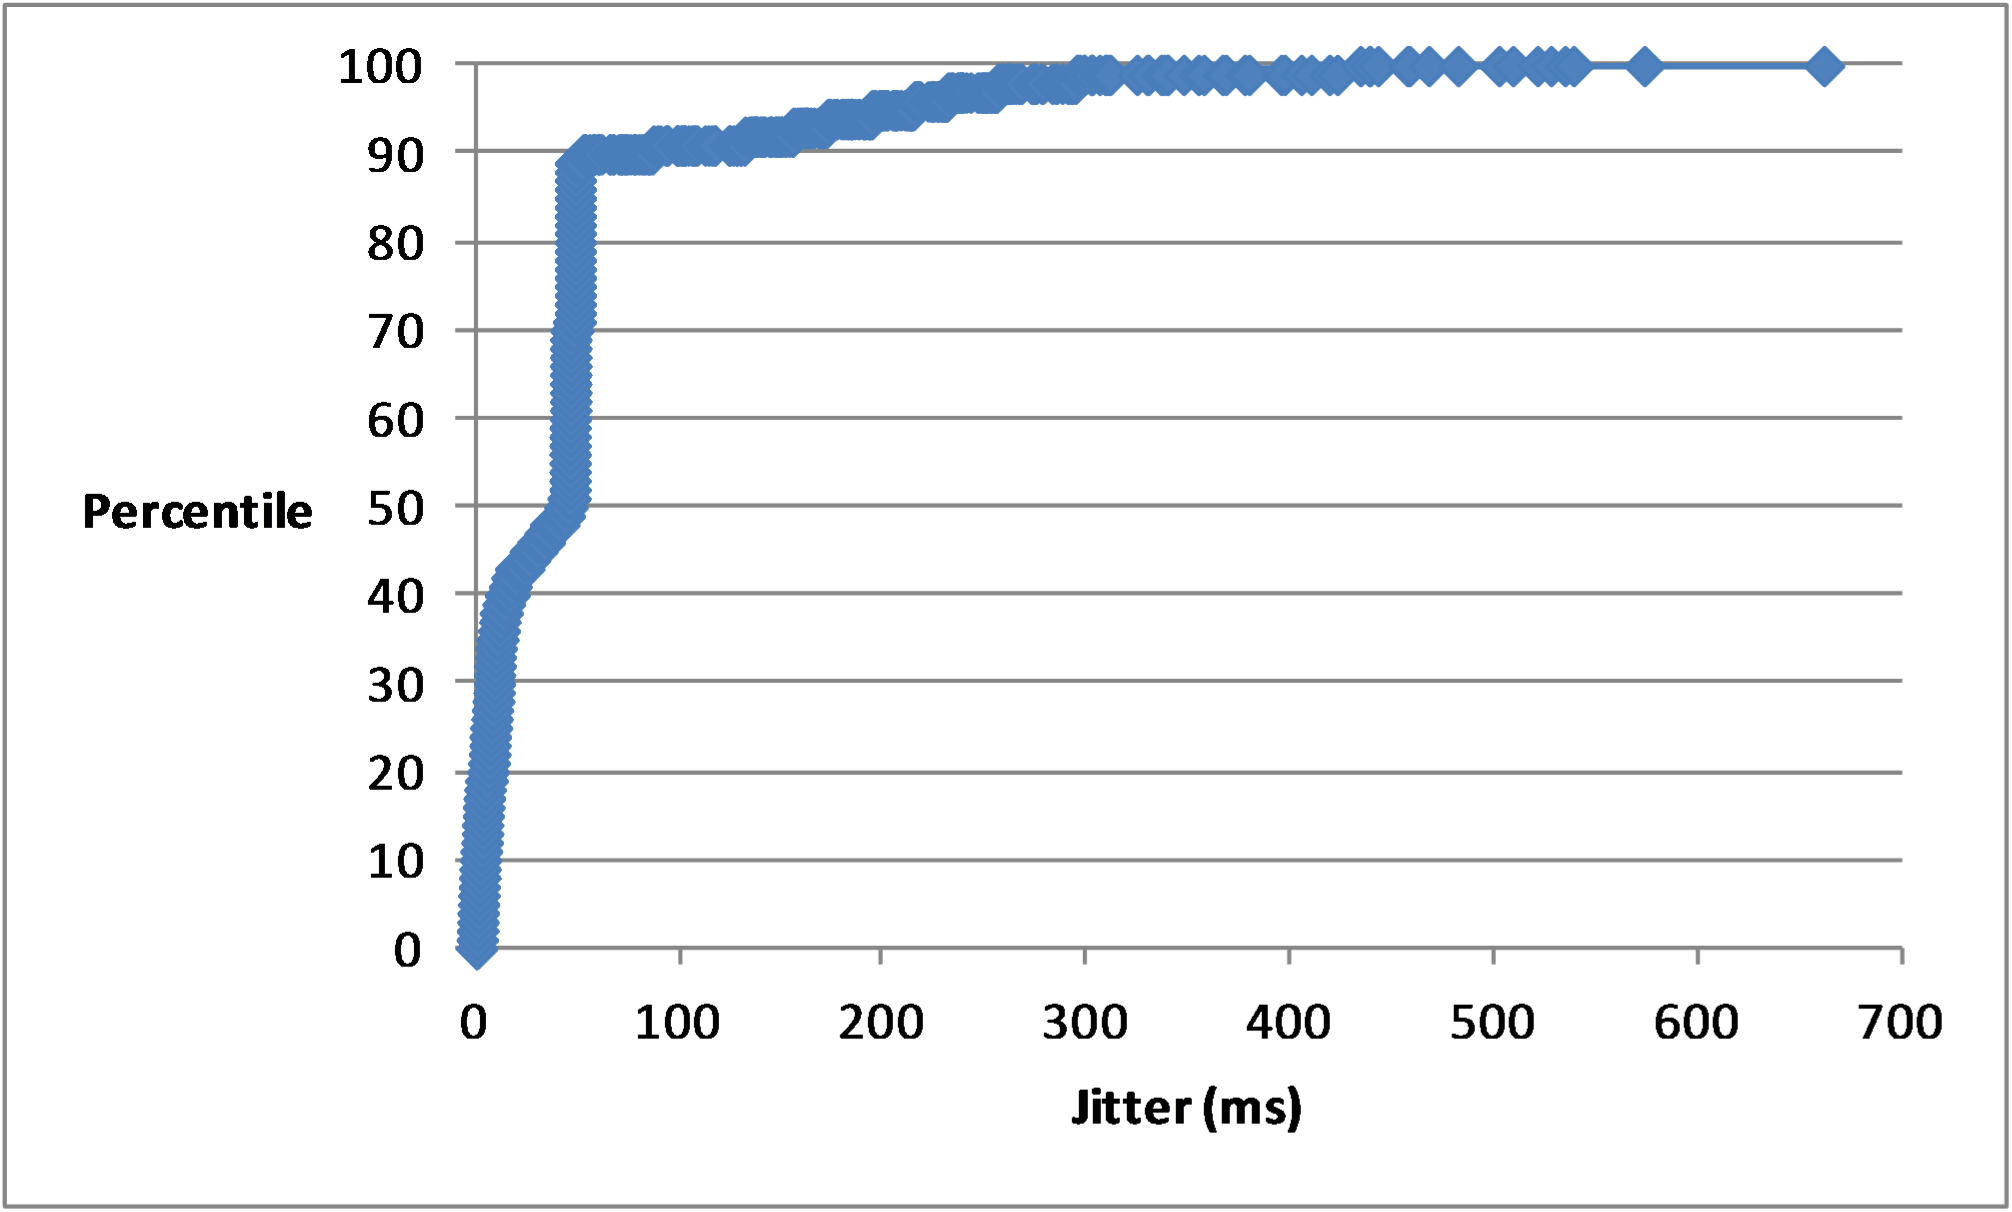
\includegraphics[width=0.45\textwidth]{pics/udp_9_jitter}
   \caption{UDP jitter CDF for 9 Mbit/s.}
\label{fig:udp_9_jitter}
\end{figure}

\begin{figure}[h]
   \centering
      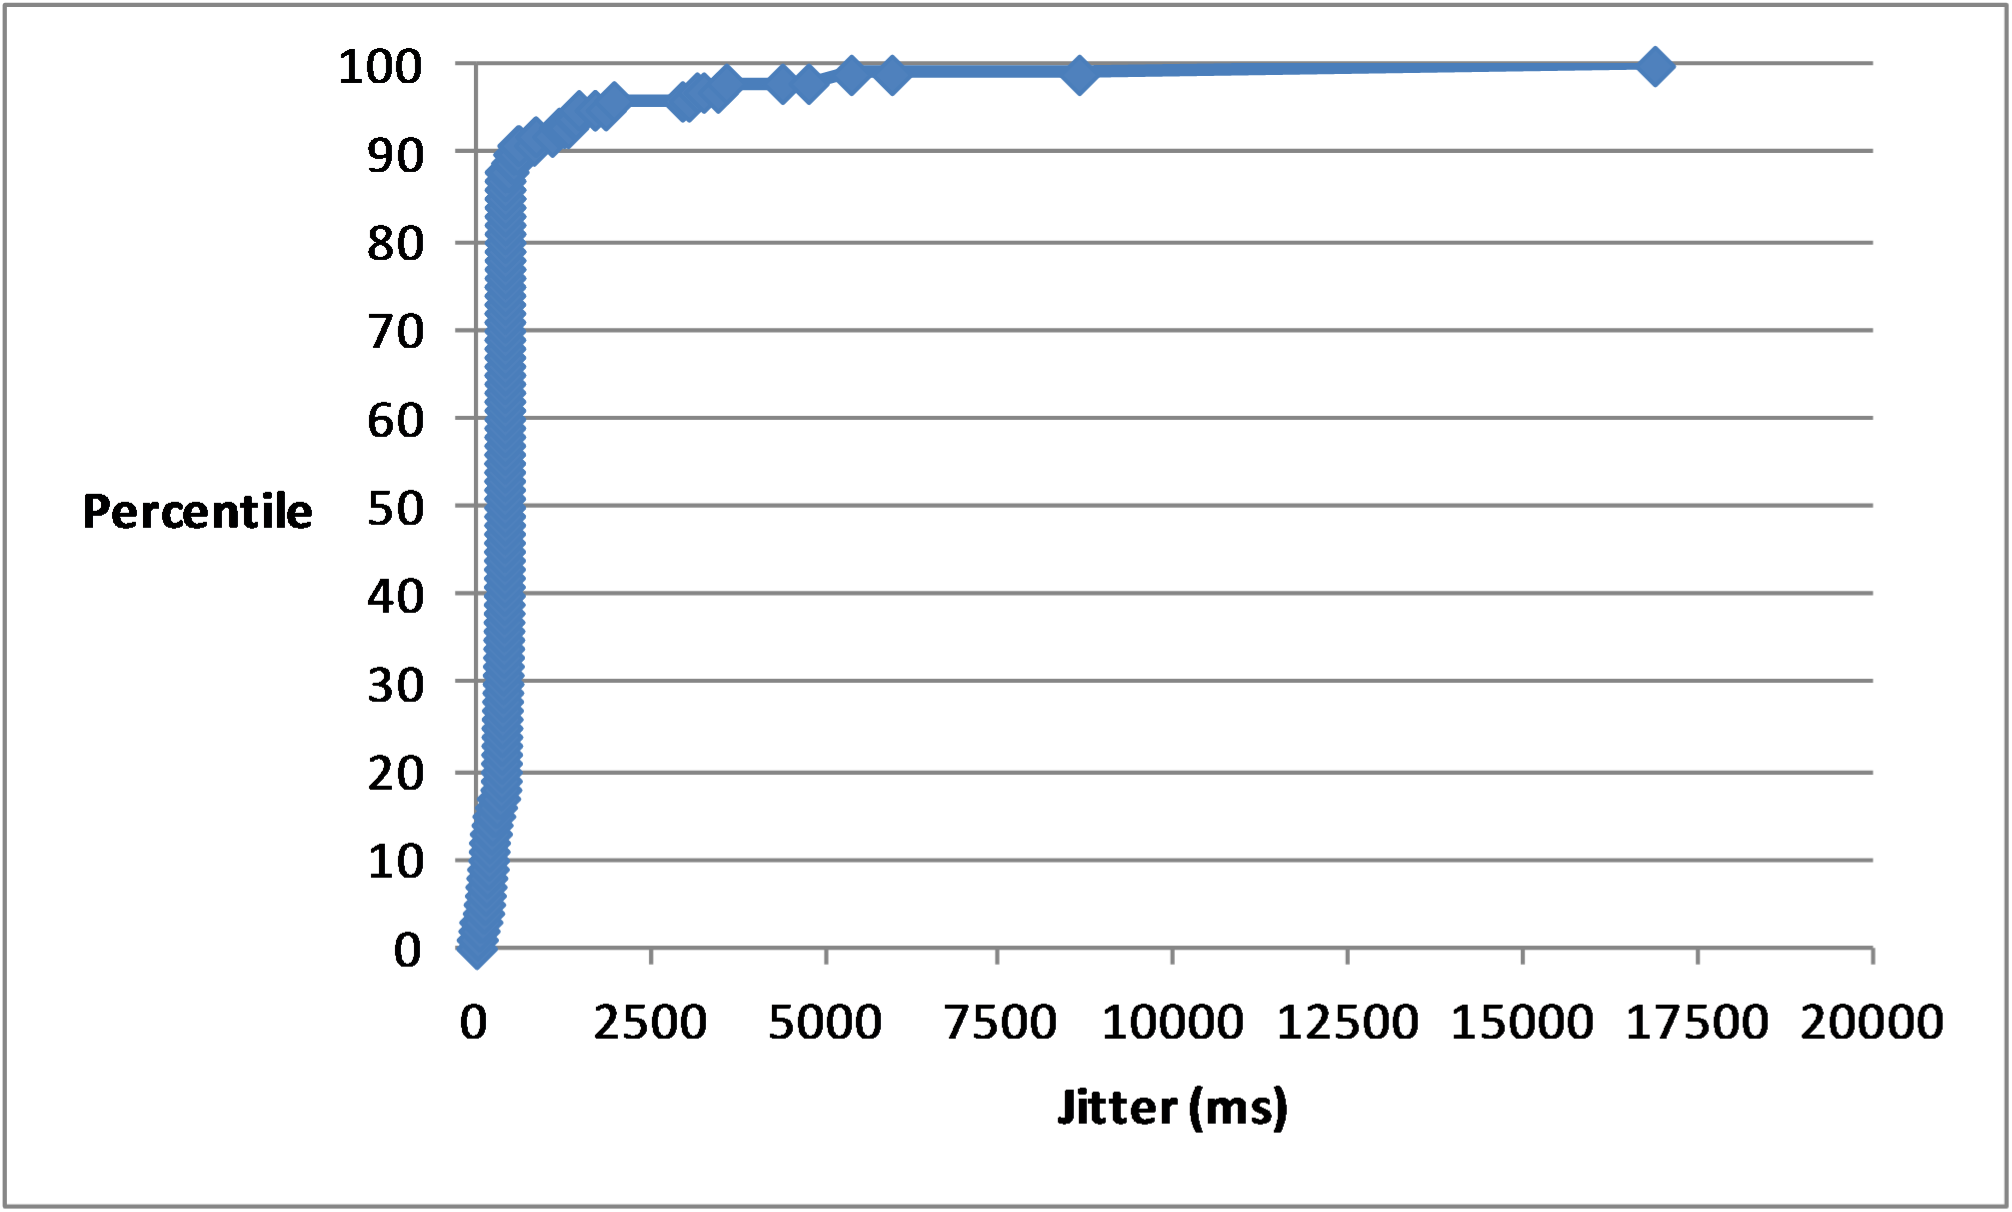
\includegraphics[width=0.45\textwidth]{pics/dccp_10_jitter_new}
   \caption{DCCP jitter CDF for 10 Mbit/s.}
\label{fig:dccp_10_jitter}
\end{figure}

\begin{figure}[h]
   \centering
      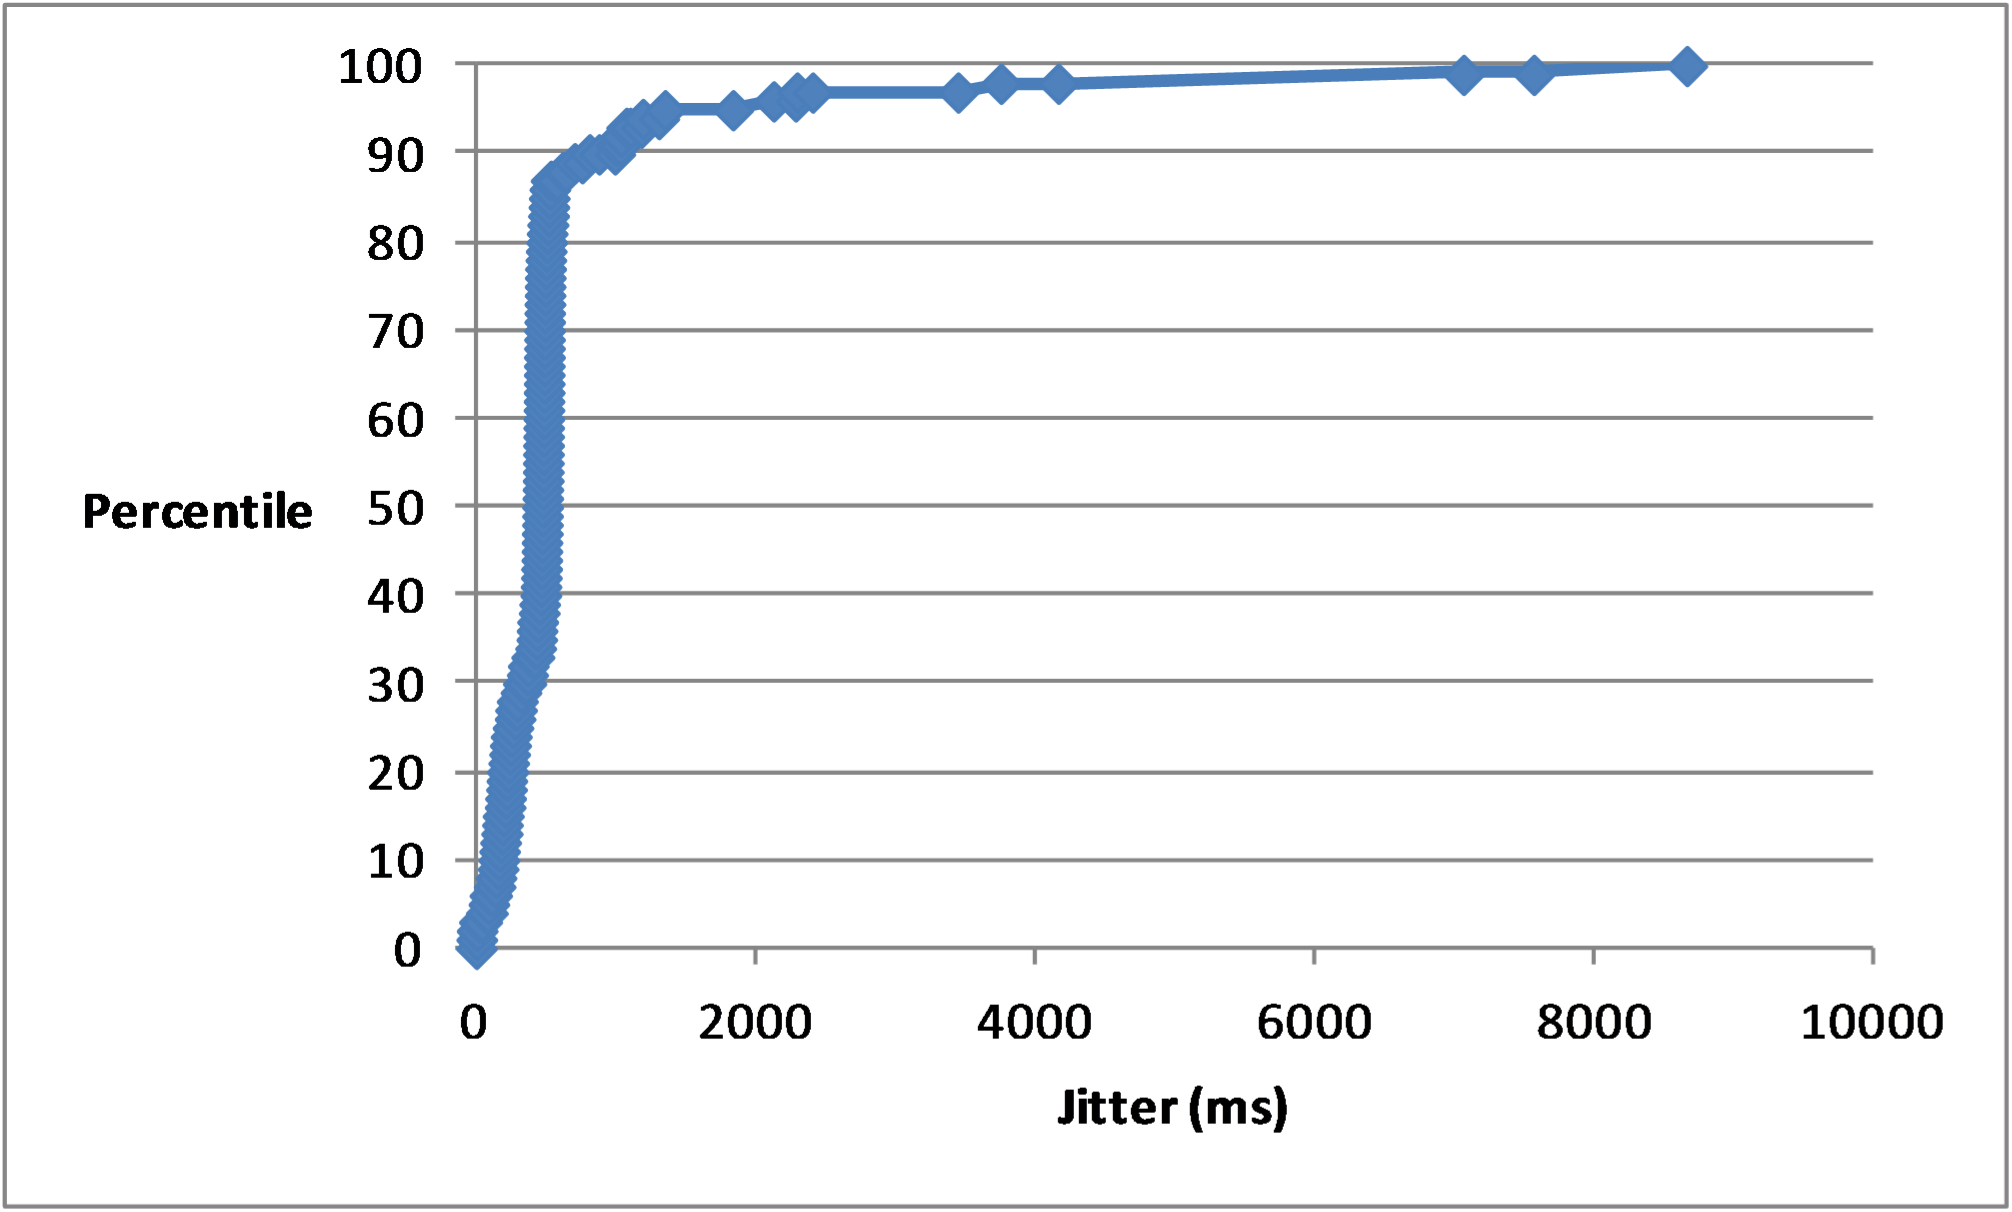
\includegraphics[width=0.45\textwidth]{pics/tcp_10_jitter}
   \caption{TCP jitter CDF for 10 Mbit/s.}
\label{fig:tcp_10_jitter}
\end{figure}

\begin{figure}[h]
   \centering
      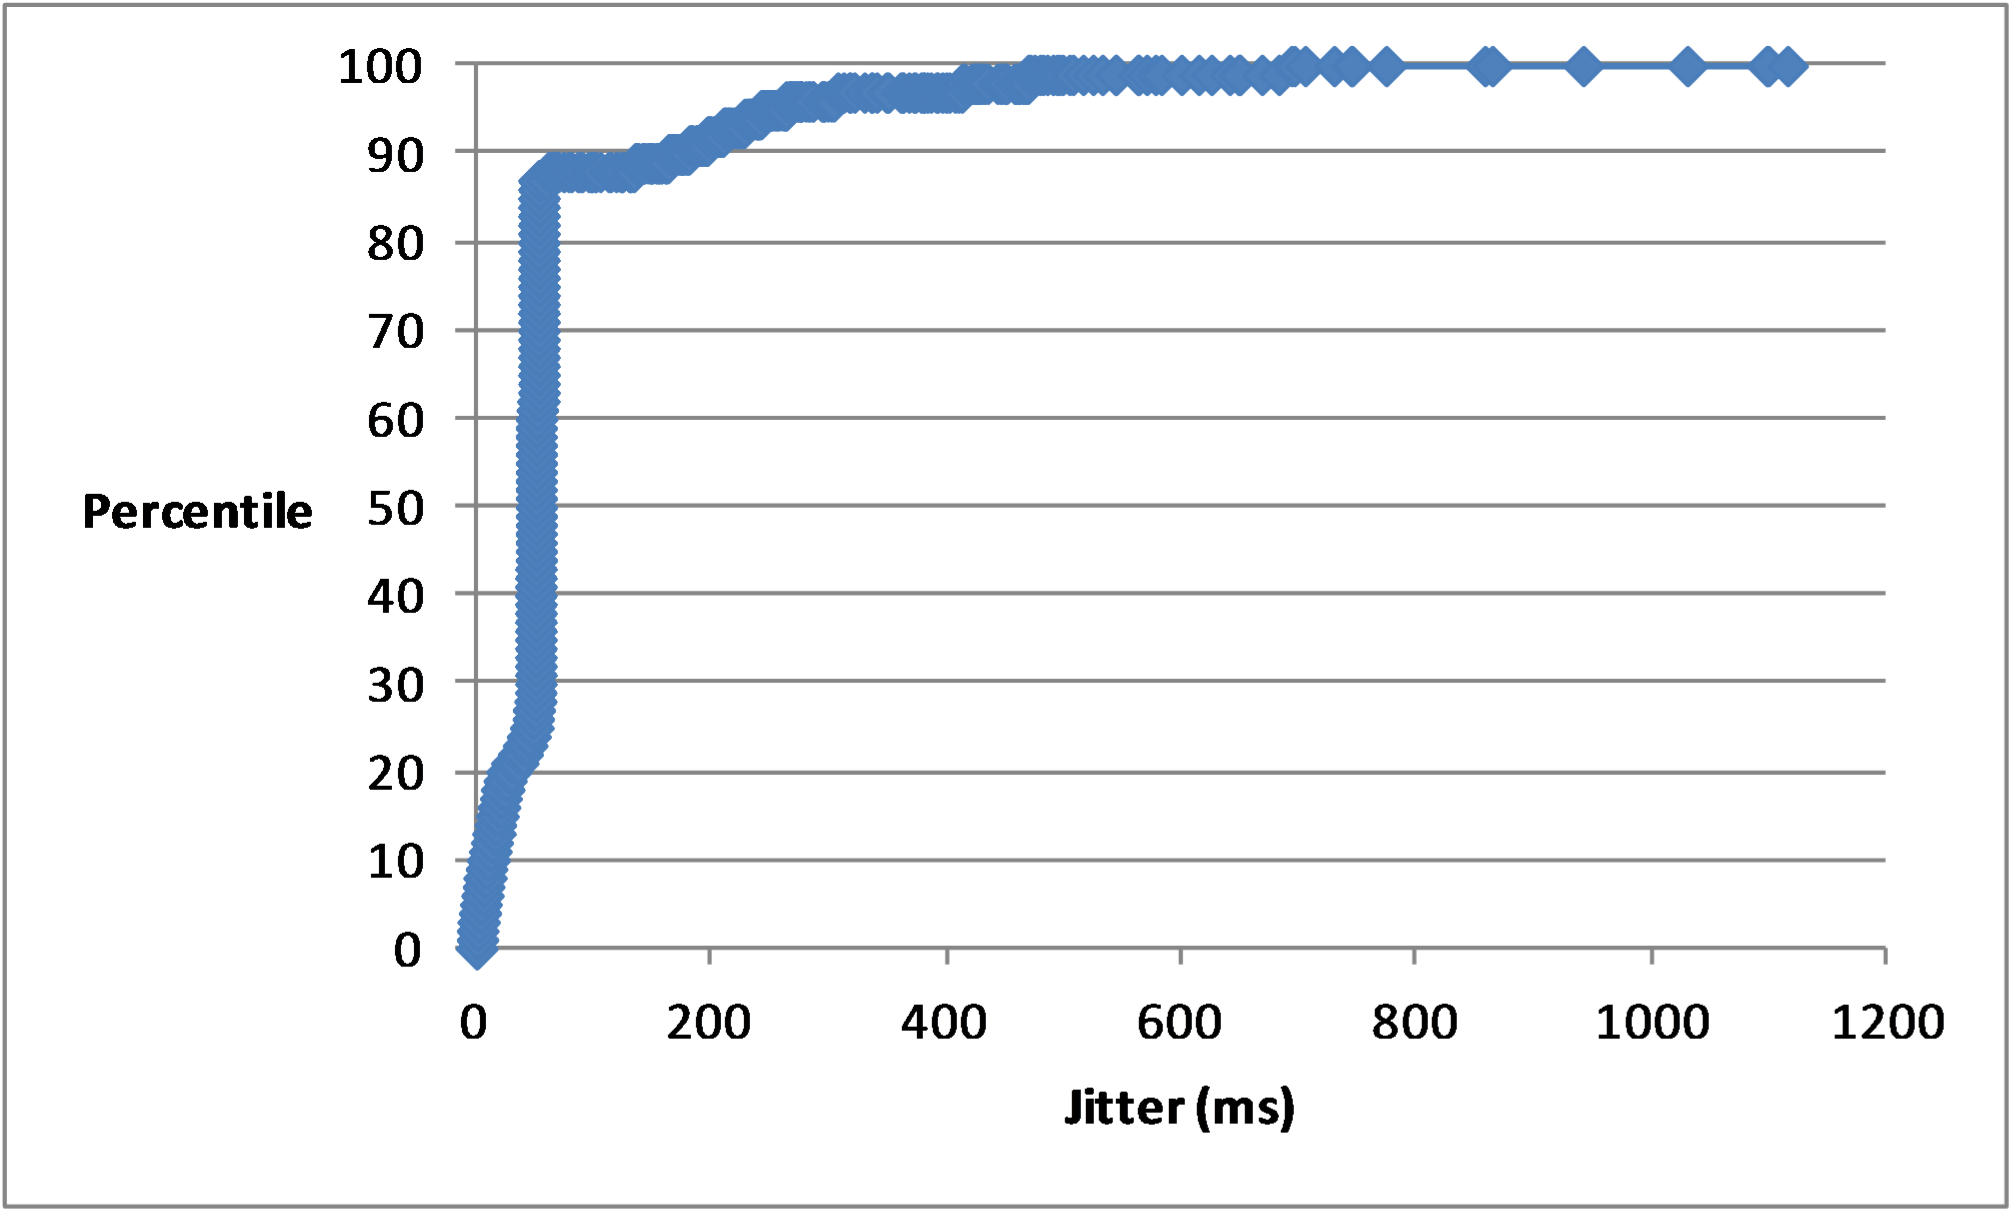
\includegraphics[width=0.45\textwidth]{pics/udp_10_jitter}
   \caption{UDP jitter CDF for 10 Mbit/s.}
\label{fig:udp_10_jitter}
\end{figure}

For TCP with no background traffic, we measured one jitter value of
approximately 5600 ms. Since no other data points were close to this outlier, we
elected to omit it to improve the graph's readability.\\

With no background traffic, all three protocols' jitter is concentrated at
approximately 5 ms, although TCP's jitter appears less uniform than that of DCCP
and UDP.\\

With 9 Mbit/s, differences begin to emerge. Approximately 90\% of DCCP's jitter
measurements are below 700 ms, with a significant majority of that 90\% lying
between roughly 600 ms and 700 ms. For TCP, about 90\% of its jitter values are
less than or equal to 500 ms, and roughly half of those measurements fall
between approximately 400 ms and 450 ms. In contrast, most of UDP's jitter
measurements at this level are at or below roughly 50 ms., and approximately
40\% fall between 40 ms and 50 ms.\\

At 10 Mbit/s, nearly 90\% of DCCP's jitter is less than about 400 ms, and
roughly 70\% is between approximately 300 ms and 400 ms. TCP's jitter is
concentrated primarily at or below 500 ms, with roughly 50\% falling between 400
ms and 500 ms. Finally, slightly over 90\% of UDP's jitter measurements are less
than 200 ms, with the majority of those values concentrated near 50 ms.\\

From this analysis, we can conclude that UDP is significantly less prone to
jitter than either DCCP or TCP during severe congestion. Since both DCCP and TCP
implement congestion control where UDP does not, it appears that congestion
control may drastically worsen jitter in such scenarios.\\

\end{document}
